
\documentclass[12pt,english]{article}
\usepackage[utf8]{inputenc}
\usepackage{tgpagella} % Palatino text only
\usepackage{mathpazo}  % Palatino math & text
\usepackage[left=1.5in,right=1.5in,top=1.5in,bottom=1.5in]{geometry}
% \linespread{1.5}
\usepackage[super,comma,sort]{natbib} % WPcomment
% \usepackage[round,sort&compress]{natbib} % NCCcomment
\usepackage{url} % [hyphens]
\usepackage[hyperpageref]{backref} % back references biblio. Needs latexmk at compilation.
\usepackage[pagebackref]{hyperref}
% \usepackage{multibib} % incompatible with backref
\hypersetup{
  colorlinks=true, % breaklinks=true,
  urlcolor=purple,    % color of external links
  linkcolor=blue,  % color of toc, list of figs etc.
  citecolor=violet,   % color of links to bibliography
}
\usepackage{bm}
\usepackage{indentfirst}
\setcitestyle{aysep={}} 
\usepackage{amsmath}
\usepackage{tcolorbox}
\usepackage{amssymb}
\usepackage{eurosym}
\usepackage{amsfonts}
\usepackage{enumerate}
\usepackage{babel}
\usepackage{graphicx}
\usepackage{caption}
\usepackage{supertabular}
\usepackage{tabularx}
\usepackage{float}
\usepackage{dsfont}
\usepackage{fancyvrb}
\usepackage{verbatim}
\usepackage{enumitem}
\usepackage{setspace}
\usepackage{comment}
\usepackage{subcaption}
\usepackage{tikz}
\usepackage{gensymb}
\usepackage{textcomp}
\usepackage{placeins} % Floats appear in their section (to use with \FloatBarrier or [section])

\usepackage{tabulary}
\usepackage{tabularx}
\usepackage{booktabs}
\usepackage{fullpage}
\usepackage{morefloats}
\usepackage{makecell}
\usepackage{lscape}
\usepackage{pdflscape}
\usepackage{longtable}
\usepackage{rotating}
\usepackage{fancyhdr}
\usepackage{tocbibind} % Adds biblio to ToC
\usepackage{tocloft}
\usepackage{titletoc} % Adds title to ToC (use with tocloft?)
\usepackage[export]{adjustbox}
\usepackage[anythingbreaks]{breakurl} % for links
\usepackage{multicol}
\newsavebox\ltmcbox % For net gain table over two columns
%\usepackage[nomarkers,figuresonly]{endfloat} % Figures at the end
%\usepackage[section,below]{placeins} % Floats placed in the section they appear in.
\renewcommand{\floatpagefraction}{.99}
\newenvironment{stretchpars}{\par\setlength{\parfillskip}{0pt}}{\par} % to justify a line


\title{Supplementary Material of\\\textit{Shortfall of Domestic Resources\\ to Eradicate Extreme Poverty by 2030}} 

% \author{Adrien Fabre$^{1,2}$} % WPcomment
\author{Adrien Fabre\footnote{CNRS, CIRED. E-mail: adrien.fabre@cnrs.fr.}}

\date{\today} % NCCcomment

\begin{document}

\sloppy
\maketitle

% \tableofcontents
% \clearpage
\listoffigures
\listoftables

\appendix % NCCcomment
\renewcommand{\thetable}{A\arabic{table}}
\renewcommand{\thefigure}{A\arabic{figure}}
\setcounter{figure}{0}
\setcounter{table}{0}

\clearpage
\section{Additional figures}

Many more figures (with varying poverty lines, taxation thresholds, growth scenarios, etc.) are available on \href{https://github.com/bixiou/domestic_poverty_eradication/tree/main/figures}{github.com/bixiou/domestic\_poverty\_eradication}. Also, any custom figure can be easily produced using this code.

% Main text figures:
% y_expropriated_2_average
% antipoverty_2_tax_7_average
% antipoverty_2_tax_18_very_optimistic
% demogrant_7__10

% Appendix figures:
% s_antipoverty_2_tax_7_average
% antipoverty_2_tax_7_reg
% antipoverty_2_tax_18_average
% s_antipoverty_2_tax_18_very_optimistic
% antipoverty_4_tax_18_average
% antipoverty_7_tax_18_average
% antipoverty_7_tax_7_average
% demogrant_7__10_very_optimistic
% s_demogrant_7__10

\begin{figure}[!htb]
  \caption[Anti-extreme-poverty tax above \$6.85/day after 3\% growth (HFCE-scaled).]{Linear tax rate above \$6.85/day eradicating extreme poverty (in \%). Data has been rescaled to match HFCE aggregate from national account. In this idealized policy, all tax revenue is transferred to the extreme poor and lift them at \$2.15/day, assuming away distorsions, and after a yearly growth of 3\% over 2022--2030. 
  }\label{fig:s_antipoverty_2_tax_7_average}
  \makebox[\textwidth][c]{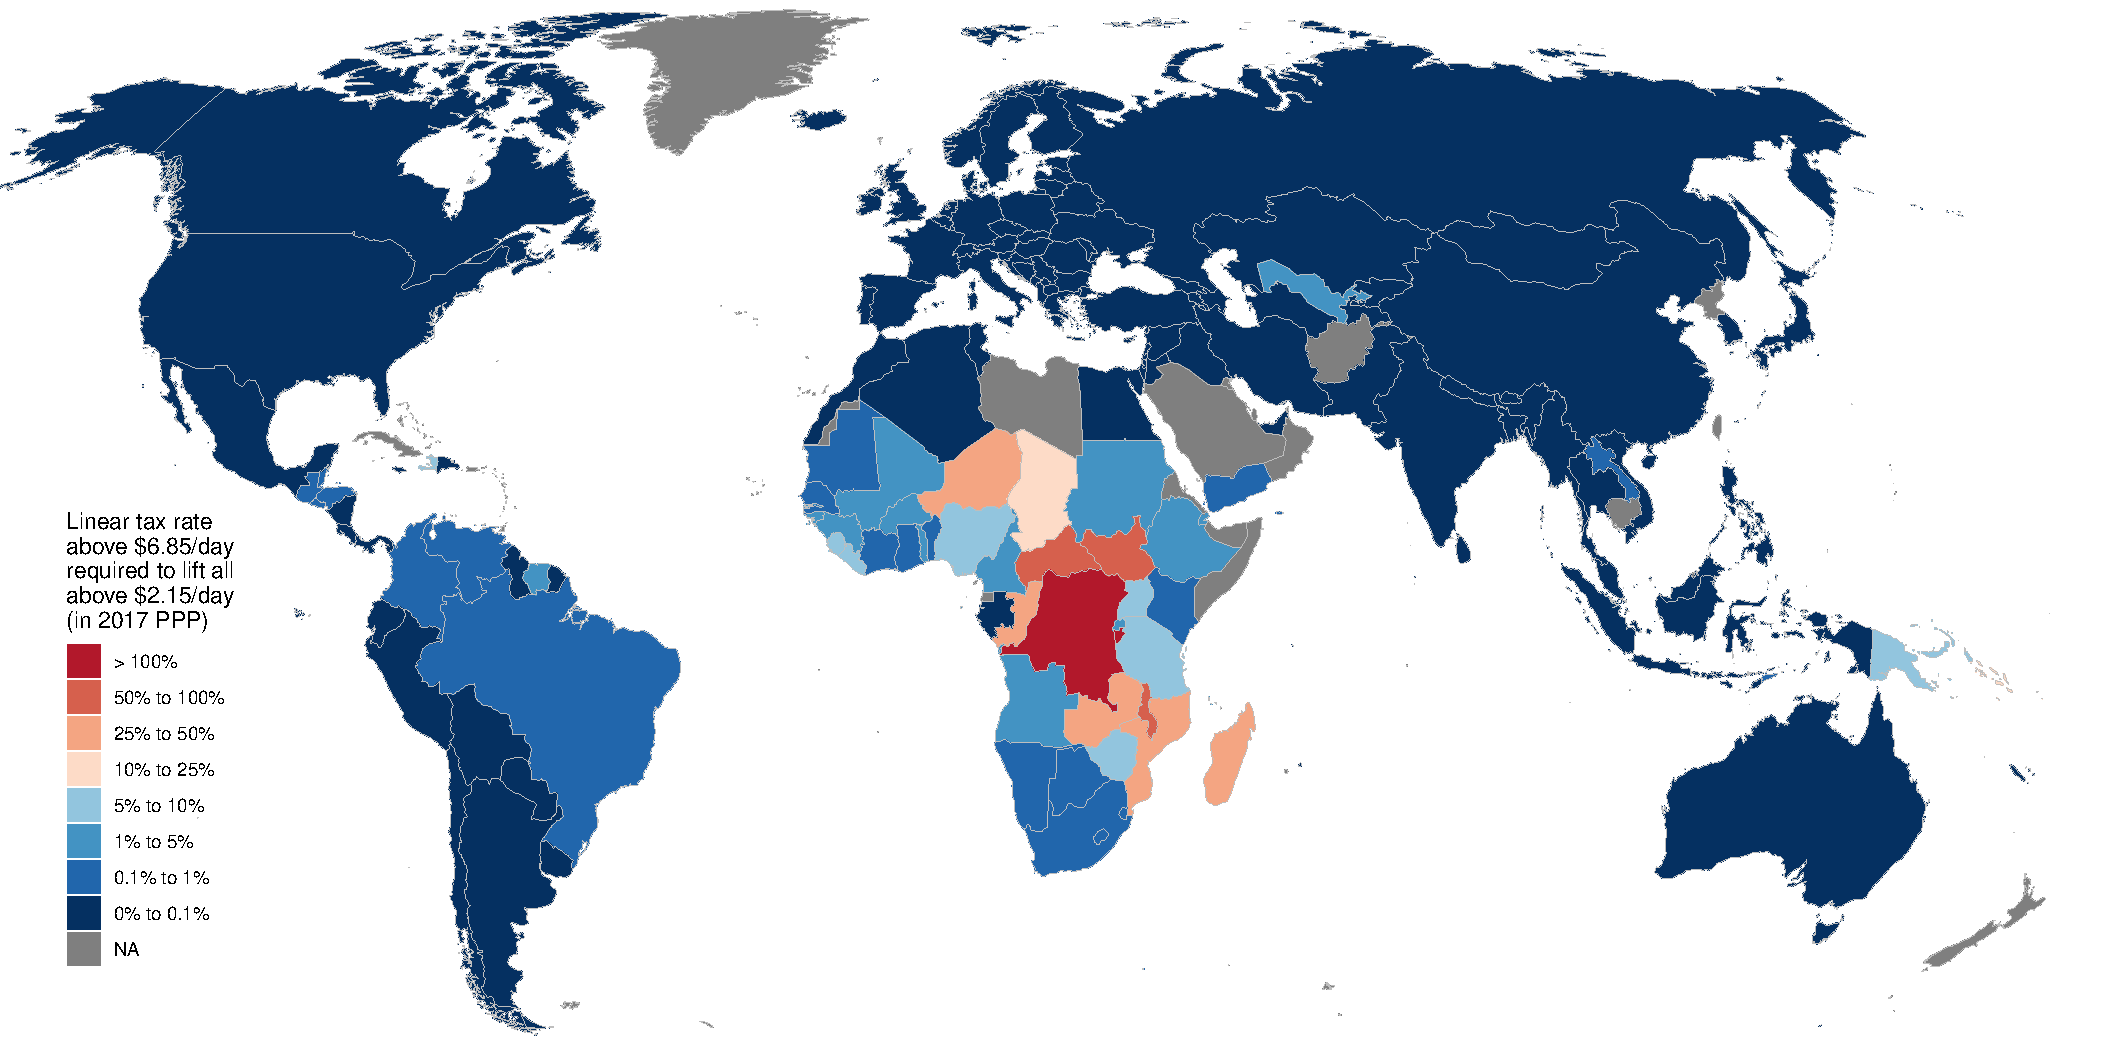
\includegraphics[width=\textwidth]
  {../figures/s_antipoverty_2_tax_7_average.pdf}}
\end{figure}

\begin{figure}[!htb]
  \caption[Anti-extreme-poverty tax above \$6.85/day after 3\% growth (HFCE-scaled).]{Linear tax rate above \$6.85/day eradicating extreme poverty (in \%). In this idealized policy, all tax revenue is transferred to the extreme poor and lift them at \$2.15/day, assuming away distorsions, with growth until 2030 predicted at the country level. 
  }\label{fig:antipoverty_2_tax_7_reg}
  \makebox[\textwidth][c]{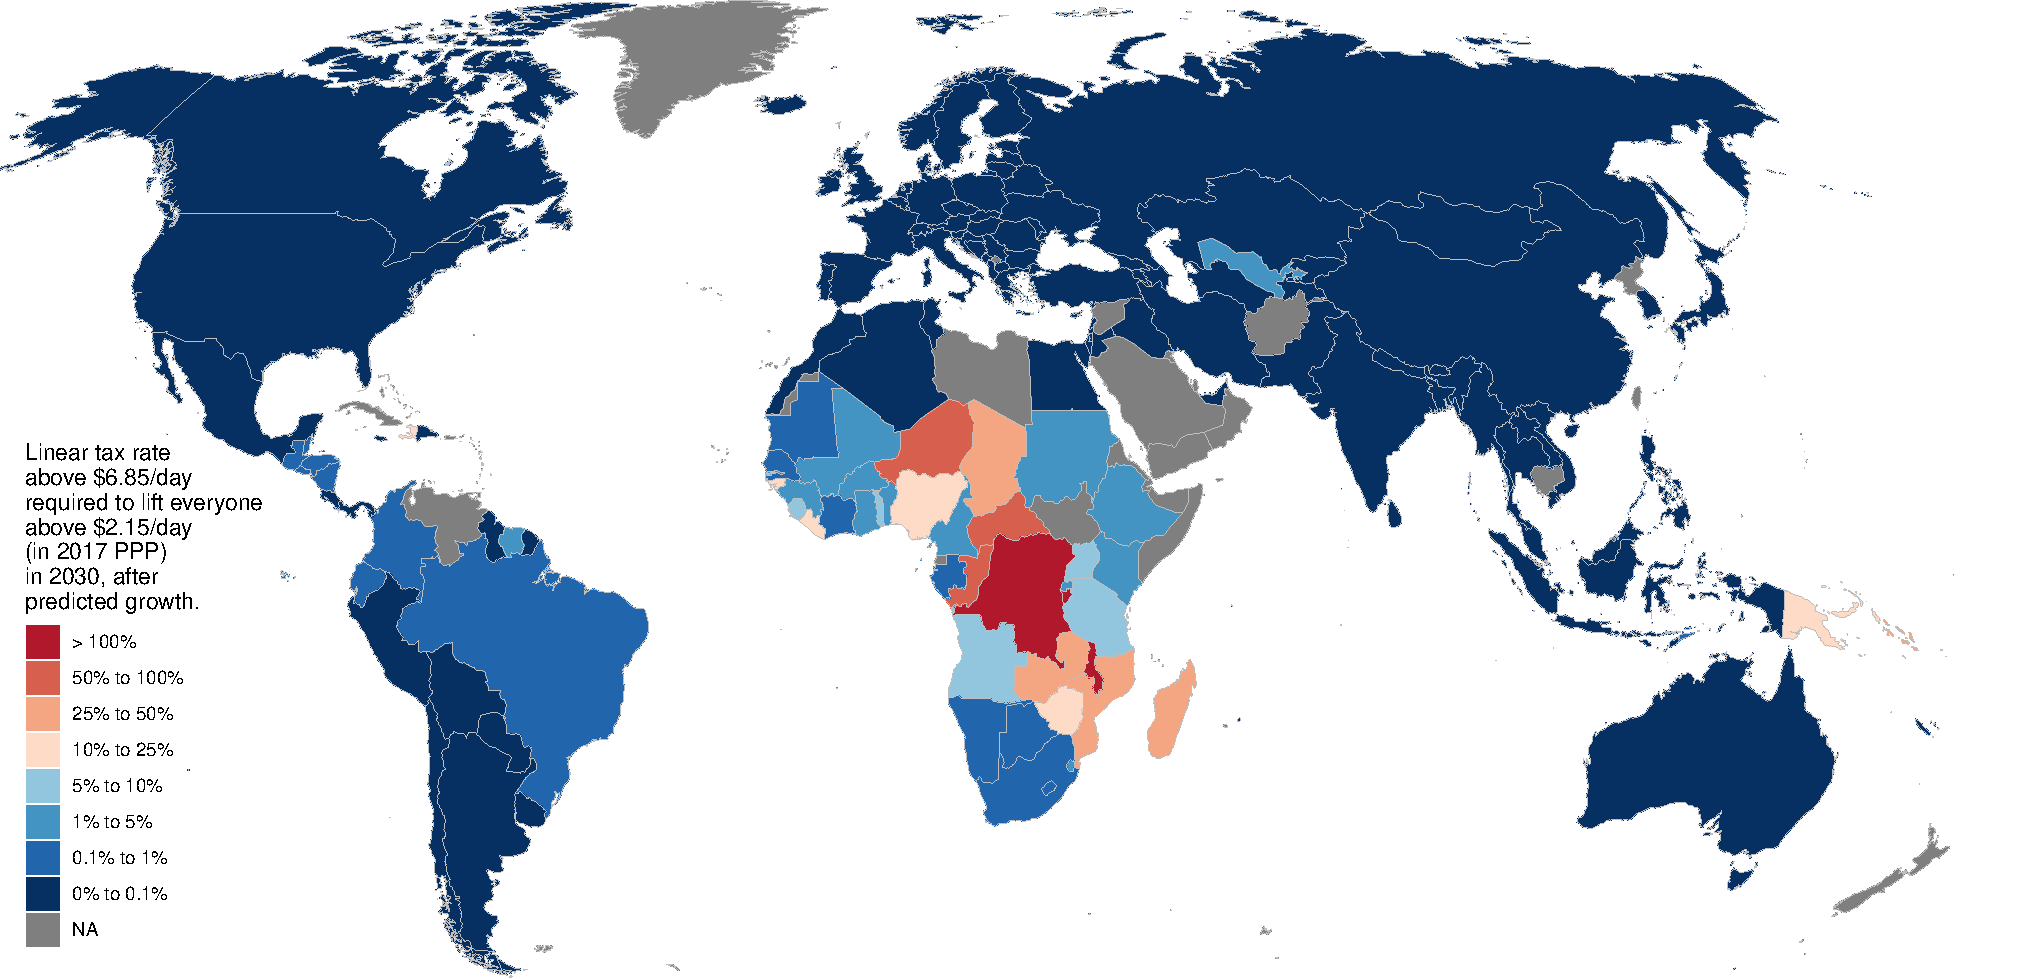
\includegraphics[width=\textwidth]
  {../figures/antipoverty_2_tax_7_reg.pdf}}
\end{figure}

\begin{figure}[!htb]
  \caption[Anti-extreme-poverty tax above \$18.15/day after 3\% growth.]{Linear tax rate above \$18.15/day eradicating extreme poverty (in \%). In this idealized policy, all tax revenue is transferred to the extreme poor and lift them at \$2.15/day, assuming away distorsions, and after a yearly growth of 3\% over 2022--2030. 
  }\label{fig:antipoverty_2_tax_18_average}
  \makebox[\textwidth][c]{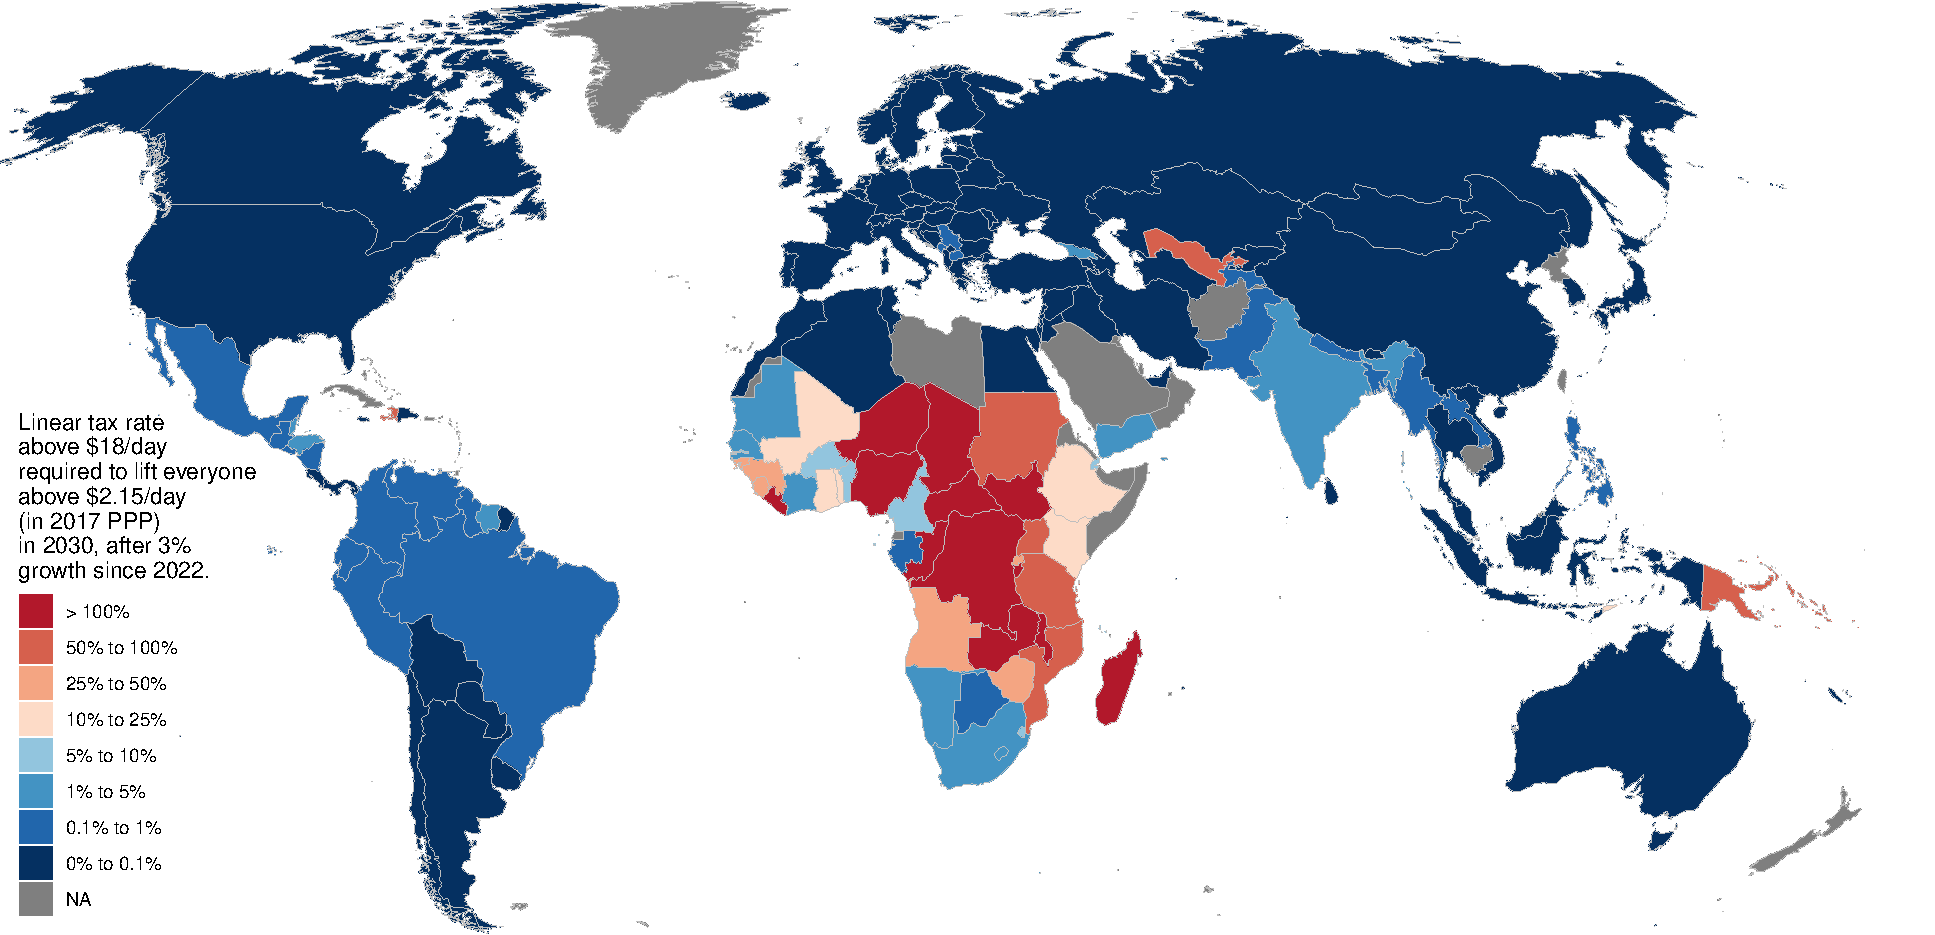
\includegraphics[width=\textwidth]
  {../figures/antipoverty_2_tax_18_average.pdf}}
\end{figure}

\begin{figure}[!htb]
  \caption[Anti-extreme-poverty tax above \$18.15/day after 7\% growth (HFCE-scaled).]{Linear tax rate above \$18.15/day eradicating extreme poverty (in \%). Data has been rescaled to match HFCE aggregate from national account. In this idealized policy, all tax revenue is transferred to the extreme poor and lift them at \$2.15/day, assuming away distorsions, and after a yearly growth of 7\% over 2022--2030. 
  }\label{fig:s_antipoverty_2_tax_18_very_optimistic}
  \makebox[\textwidth][c]{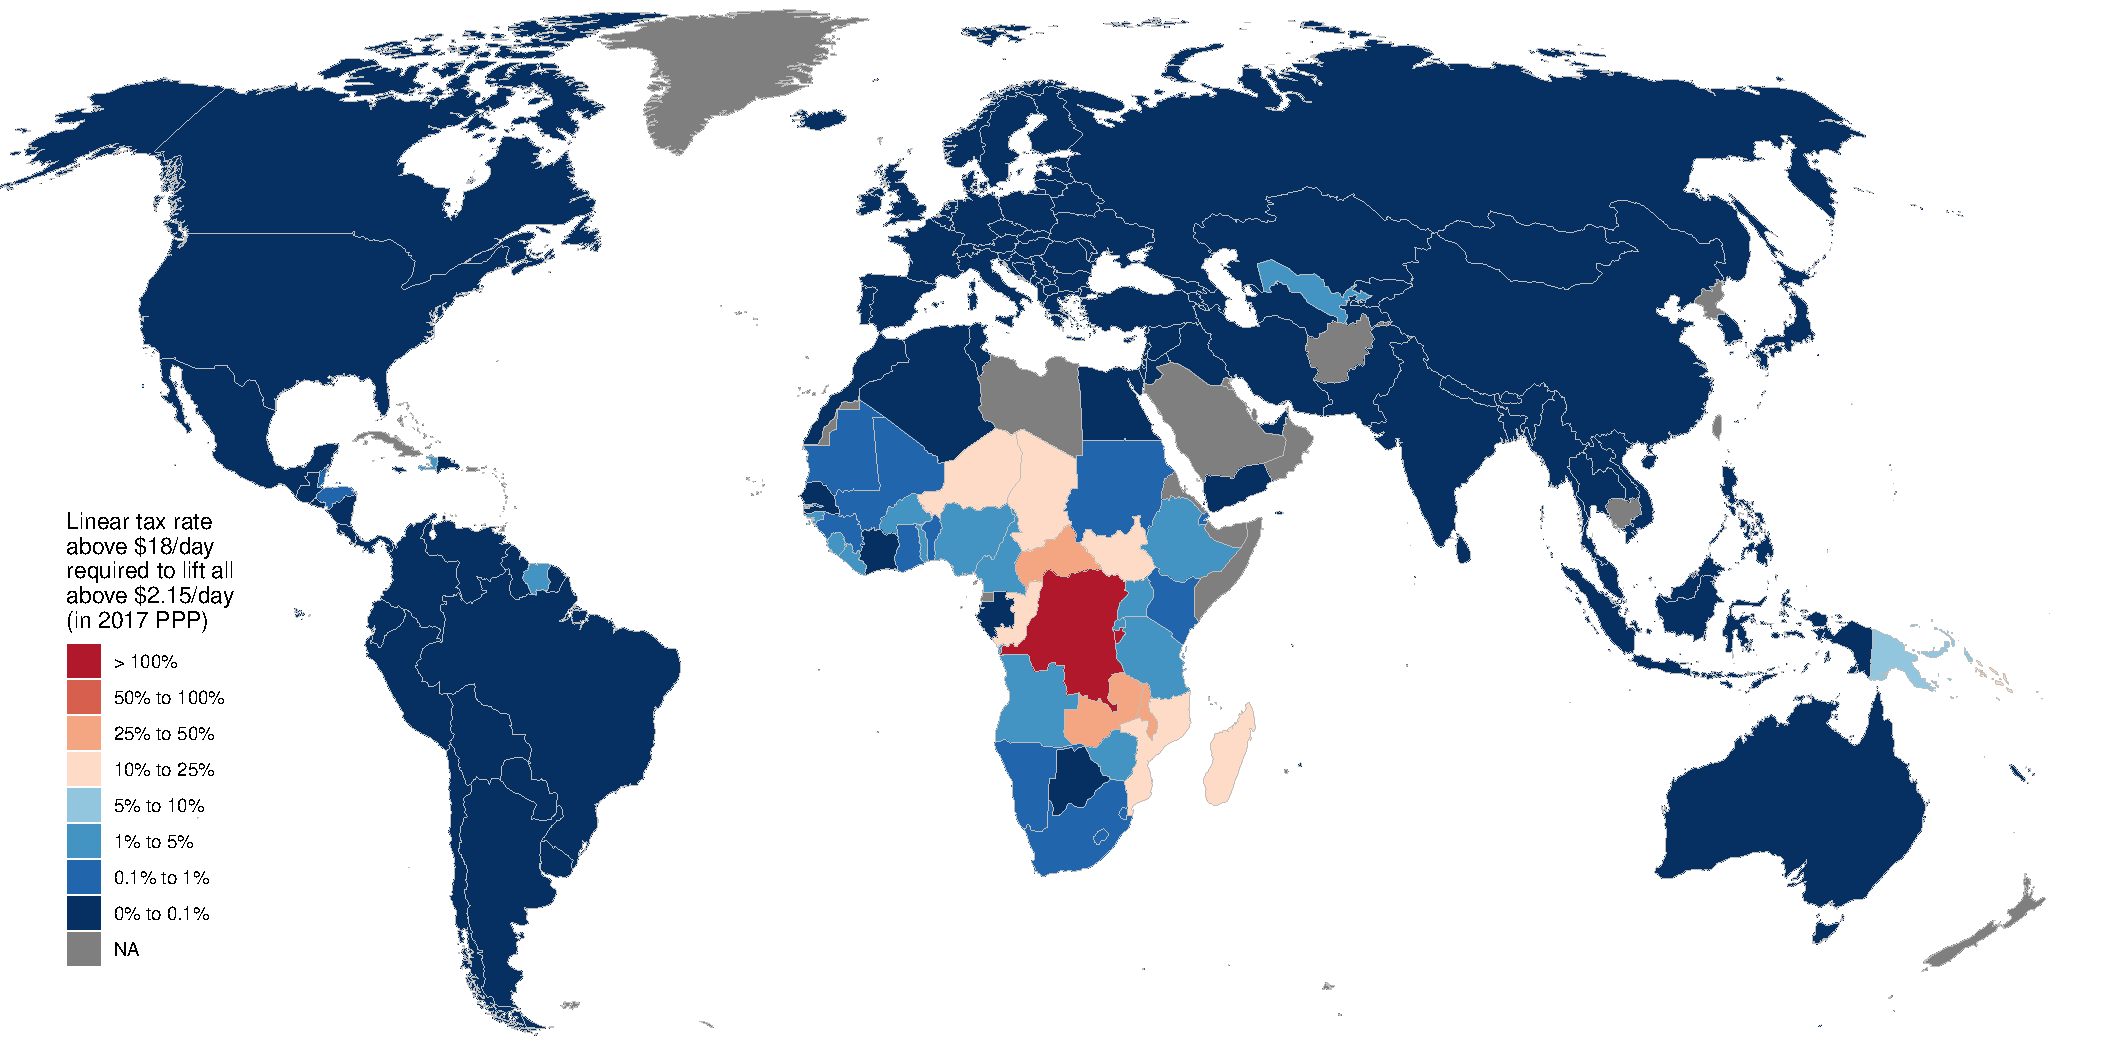
\includegraphics[width=\textwidth]
  {../figures/s_antipoverty_2_tax_18_very_optimistic.pdf}}
\end{figure}

\begin{figure}[!htb]
  \caption[Anti-severe-poverty tax above \$18.15/day after 3\% growth (HFCE-scaled).]{Linear tax rate above \$18.15/day eradicating extreme poverty (in \%). In this idealized policy, all tax revenue is transferred to the extreme poor and lift them at \$3.65/day, assuming away distorsions, and after a yearly growth of 3\% over 2022--2030. 
  }\label{fig:antipoverty_4_tax_18_average}
  \makebox[\textwidth][c]{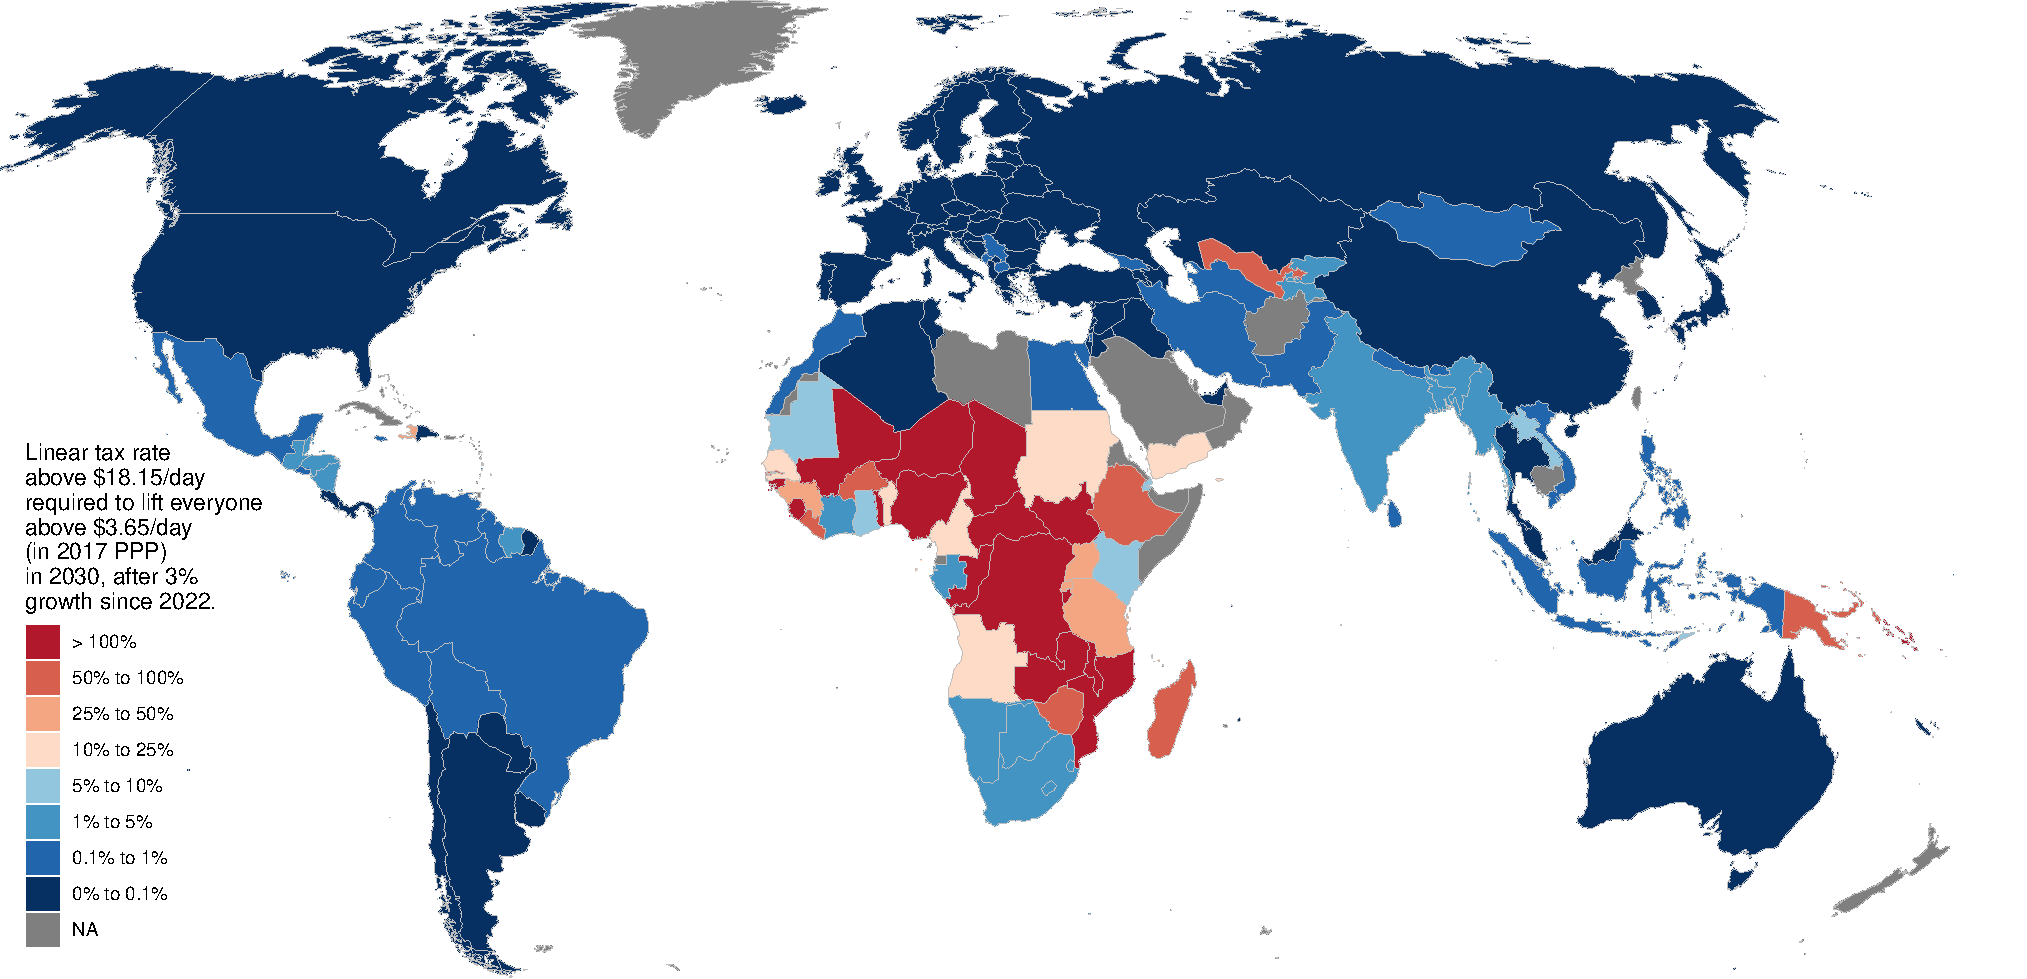
\includegraphics[width=\textwidth]
  {../figures/antipoverty_4_tax_18_average.pdf}}
\end{figure}

\begin{figure}[!htb]
  \caption[Anti-acute-poverty tax above \$18.15/day after 3\% growth (HFCE-scaled).]{Linear tax rate above \$18.15/day eradicating extreme poverty (in \%). In this idealized policy, all tax revenue is transferred to the extreme poor and lift them at \$6.85/day, assuming away distorsions, and after a yearly growth of 3\% over 2022--2030. 
  }\label{fig:antipoverty_7_tax_18_average}
  \makebox[\textwidth][c]{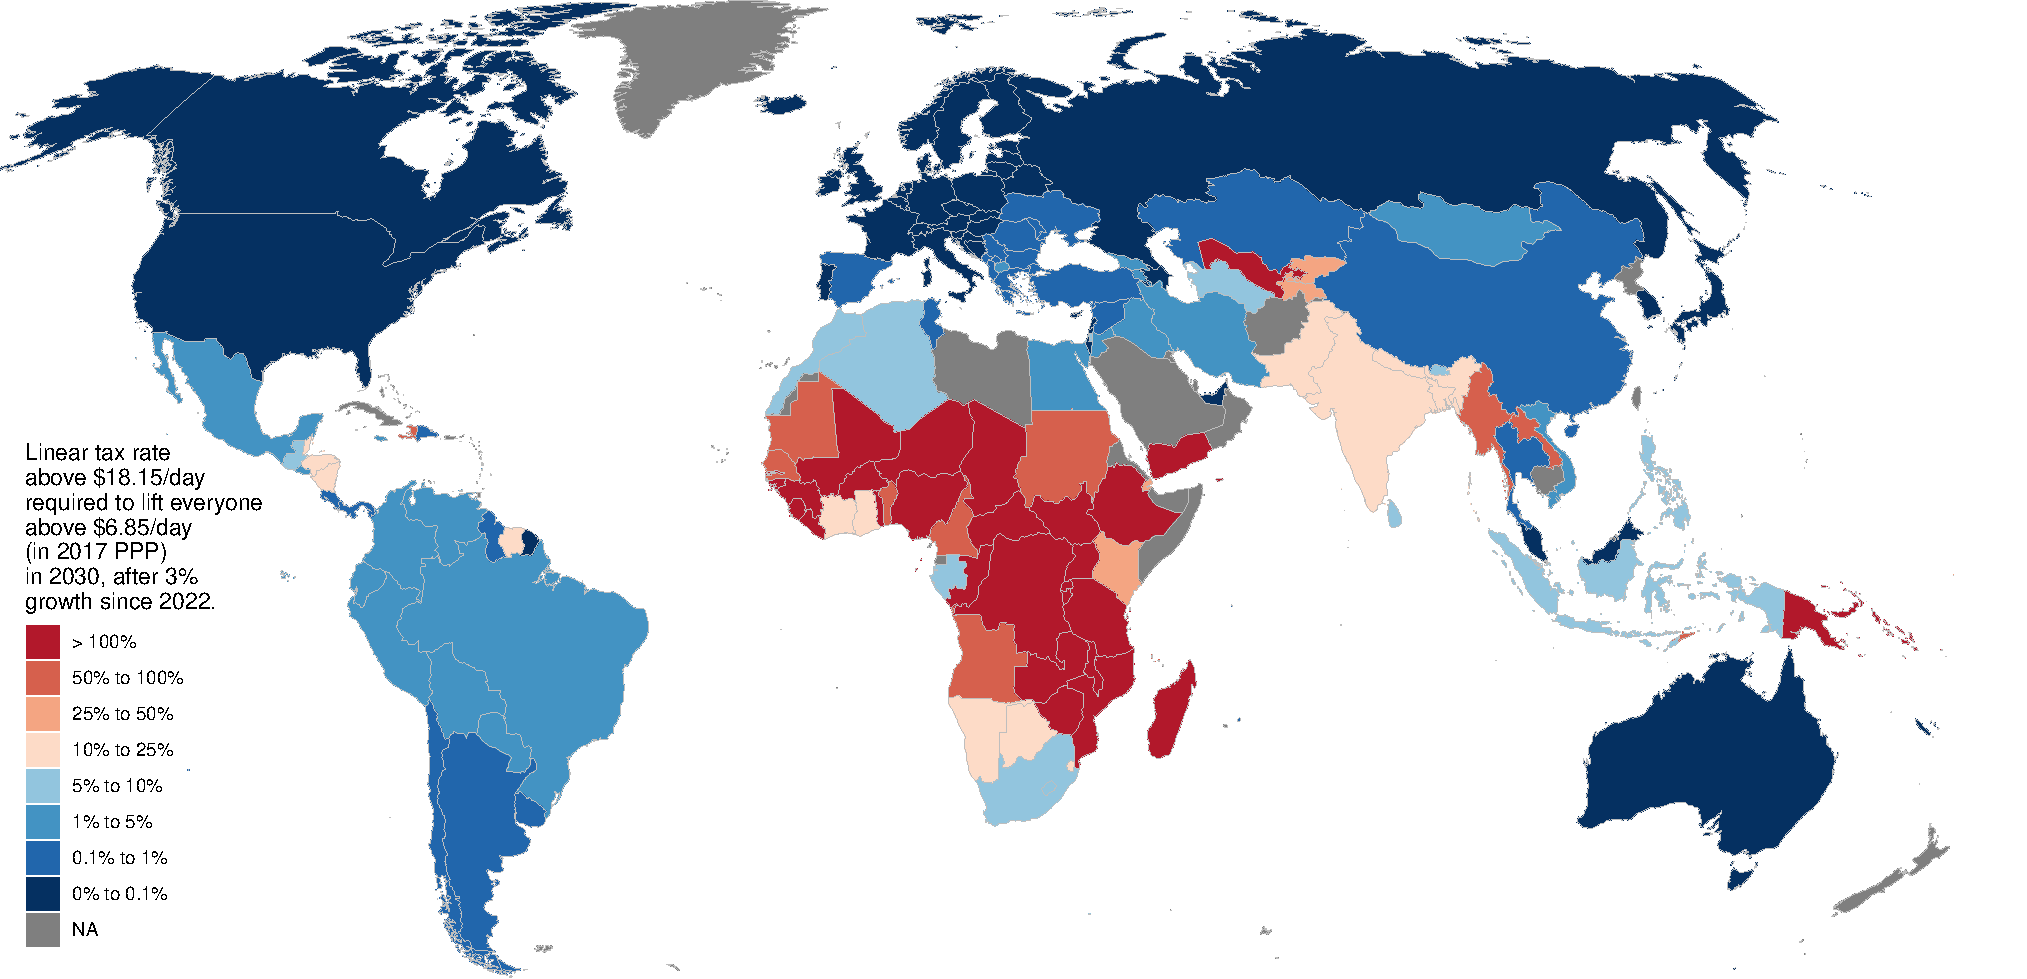
\includegraphics[width=\textwidth]
  {../figures/antipoverty_7_tax_18_average.pdf}}
\end{figure}

\begin{figure}[!htb]
  \caption[Anti-acute-poverty tax above \$6.85/day after 3\% growth (HFCE-scaled).]{Linear tax rate above \$6.85/day eradicating extreme poverty (in \%). In this idealized policy, all tax revenue is transferred to the extreme poor and lift them at \$6.85/day, assuming away distorsions, and after a yearly growth of 3\% over 2022--2030. 
  }\label{fig:antipoverty_7_tax_7_average}
  \makebox[\textwidth][c]{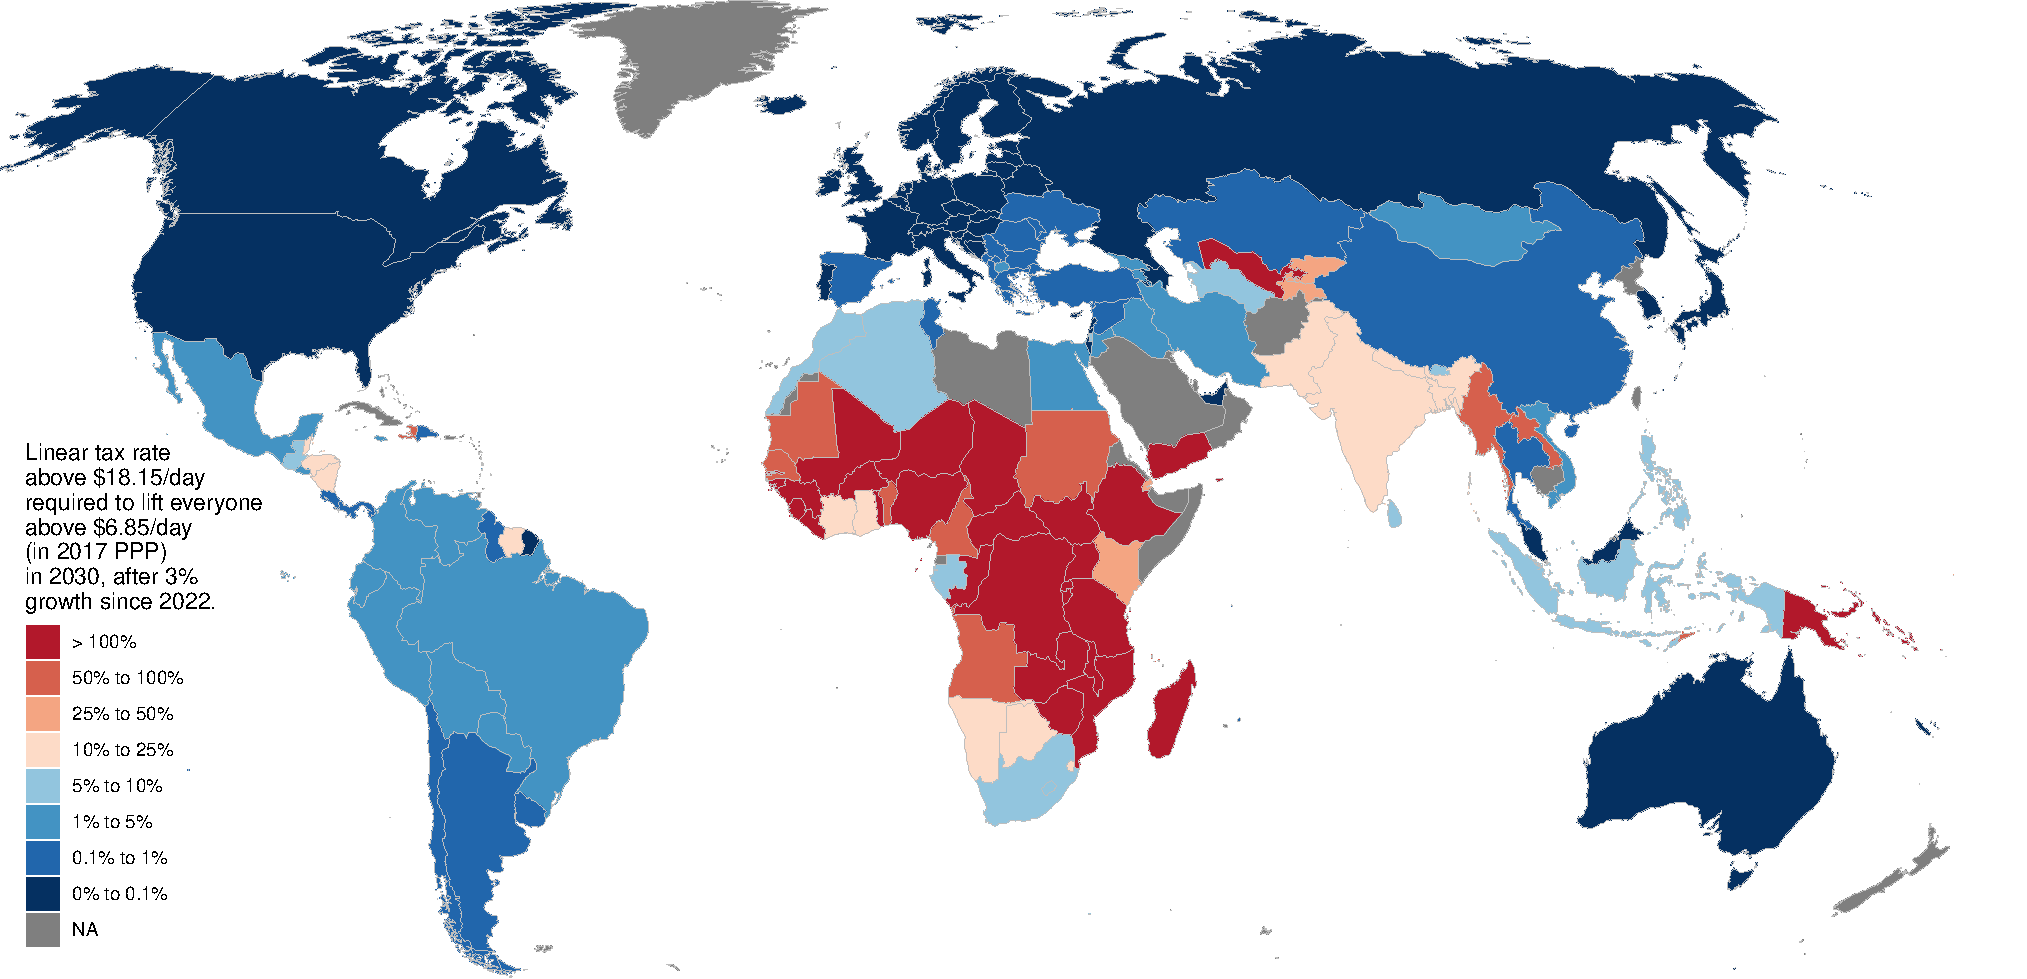
\includegraphics[width=\textwidth]
  {../figures/antipoverty_7_tax_7_average.pdf}}
\end{figure}

\begin{figure}[!htb]
  \caption[Income floor of 10\% tax above \$6.85/day after 7\% growth.]{Income floor that can be funded with a 10\% marginal tax on income above \$6.85/day (in 2017 PPP \$/day). In this idealized policy, all tax revenue is transferred to the poorest and lift them at the income floor, assuming away distorsions, and after a yearly growth of 7\% over 2022--2030. 
  }\label{fig:demogrant_7__10_very_optimistic}
  \makebox[\textwidth][c]{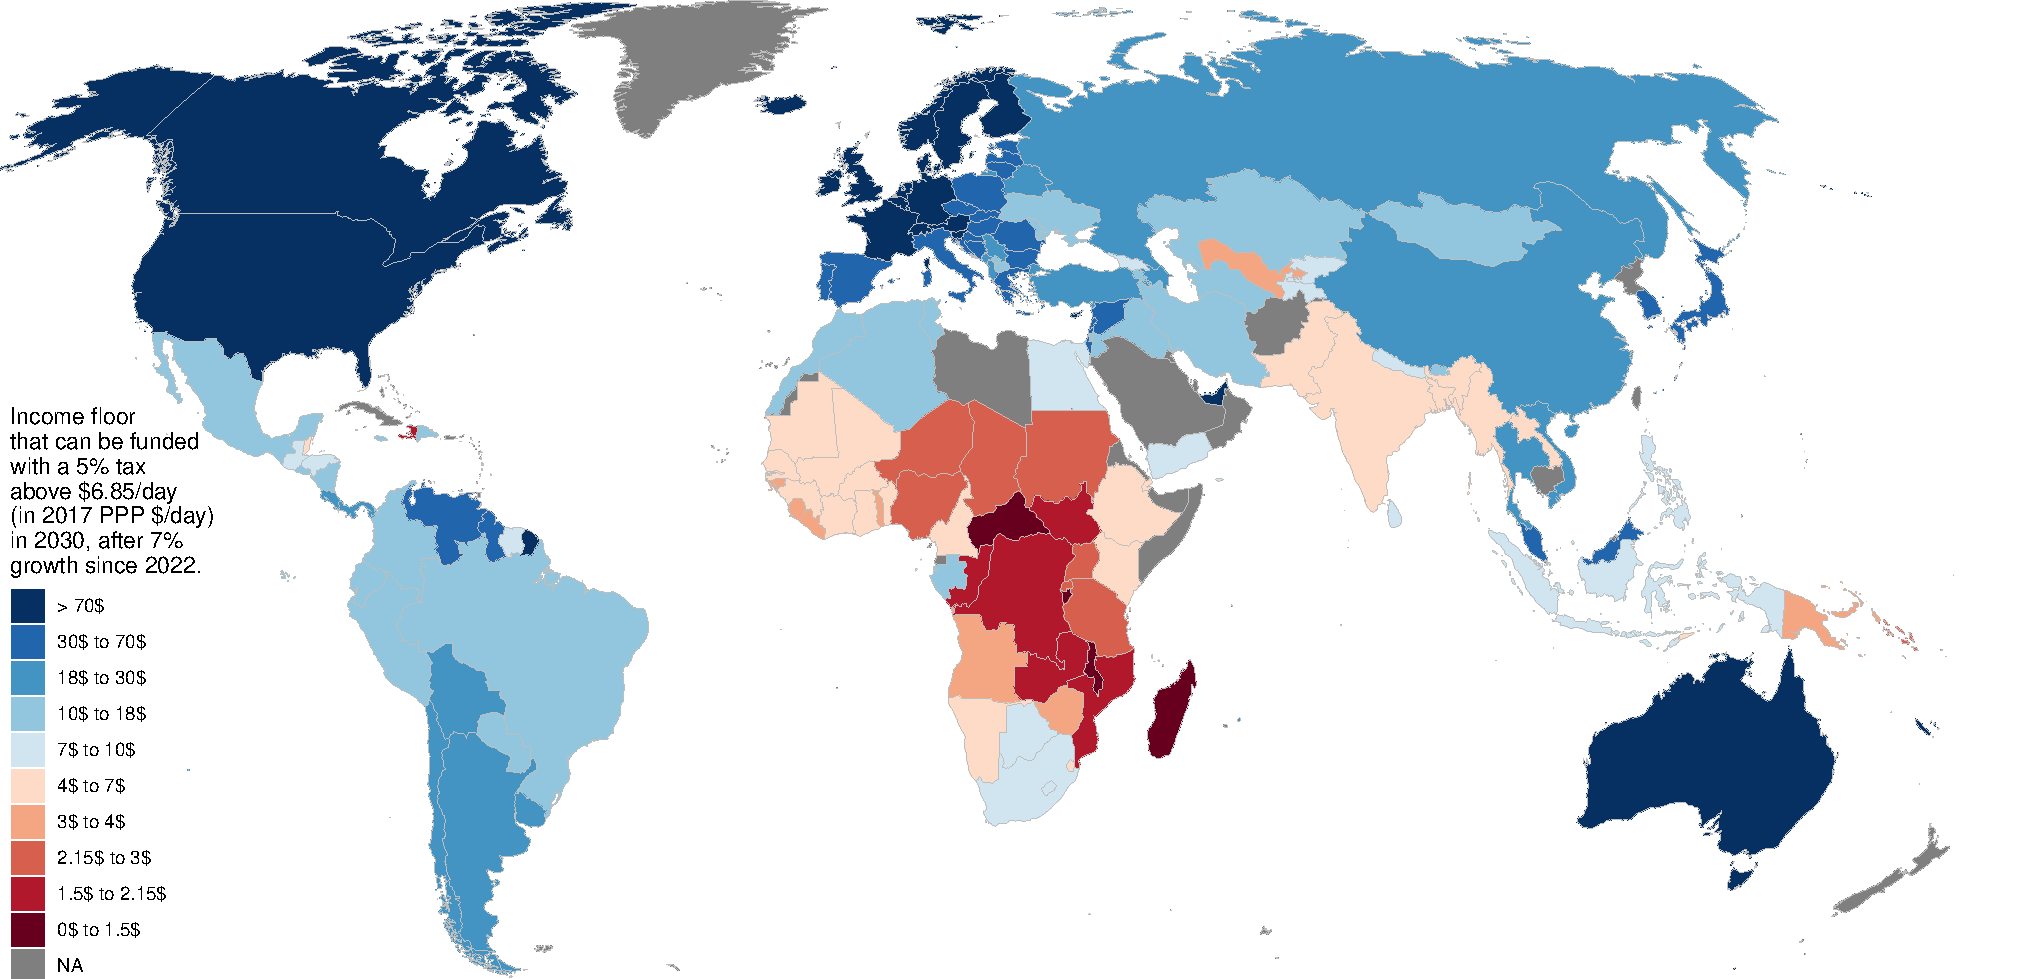
\includegraphics[width=\textwidth]
  {../figures/demogrant_7__10_very_optimistic.pdf}}
\end{figure}

\FloatBarrier
\begin{figure}[!htb]
  \caption[Income floor of 10\% tax above \$6.85/day after 3\% growth (HFCE-scaled).]{Income floor that can be funded with a 10\% marginal tax on income above \$6.85/day (in 2017 PPP \$/day). Data has been rescaled to match HFCE aggregate from national account. In this idealized policy, all tax revenue is transferred to the poorest and lift them at the income floor, assuming away distorsions, and after a yearly growth of 3\% over 2022--2030. 
  }\label{fig:s_demogrant_7__10}
  \makebox[\textwidth][c]{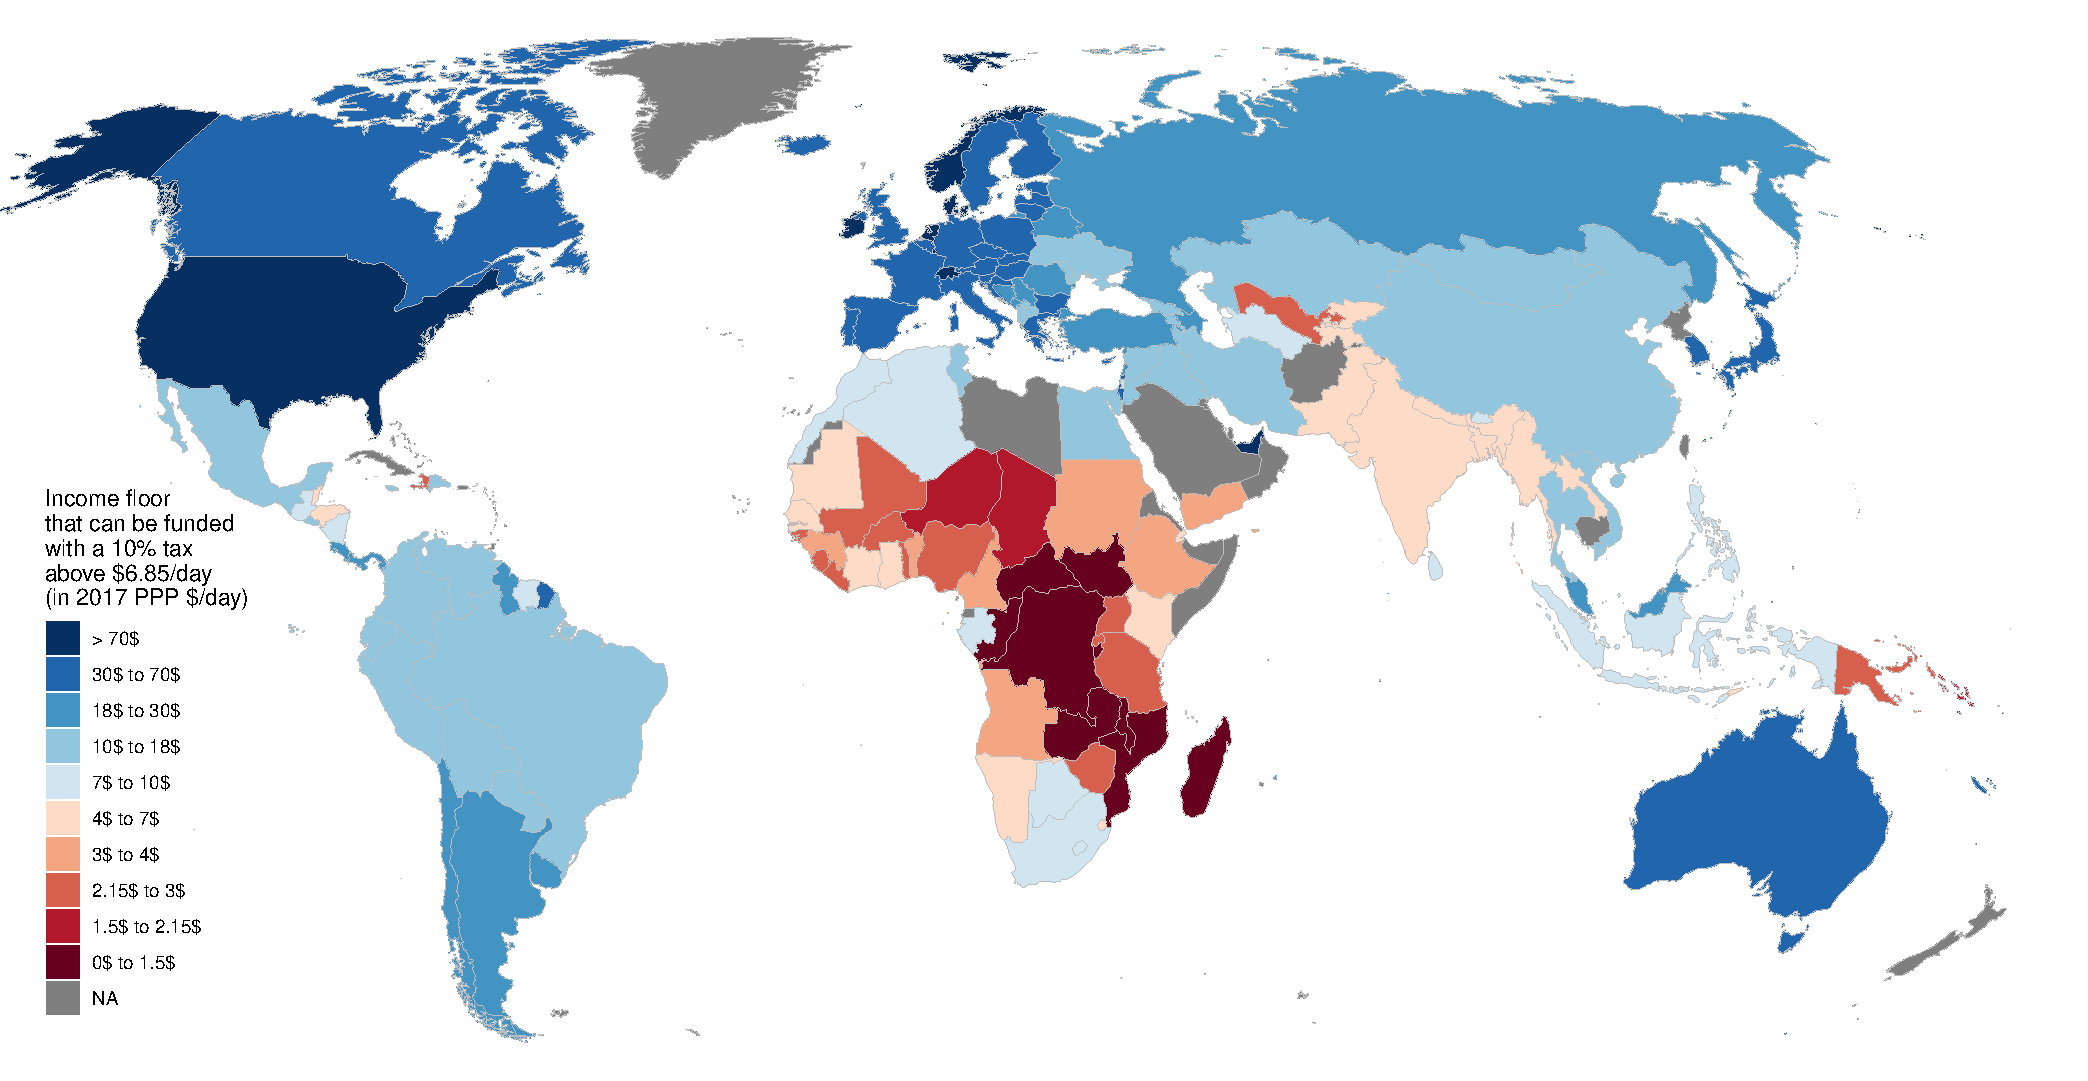
\includegraphics[width=\textwidth]
  {../figures/s_demogrant_7__10.pdf}}
\end{figure}

\section{Additional tables}
\begin{table}[b]

\caption[Mean income in different scenarios, survey years and HFCE rescaling factor.]{\label{tab:tax}Mean income for major countries in various years and growth scenarios, survey years and factor used to rescale incomes to national accounts (in countries with HFCE to survey ratio above 1).}
\makebox[\textwidth][c]{
\begin{tabular}[t]{lccccccccc}
\toprule  & Year & \multicolumn{6}{c}{Mean consumption/income (in \$/day)} & BCL & HFCE to  \\ 
 Indicator & of & year of & 2022 & \multicolumn{4}{c}{2030 estimate} & survey & survey \\ 
 & Survey & survey & est. & 3\% & 7\% & Projection & Trend & year & ratio \\ 
\midrule
World & 2018 & 17.2 & 18.6 & 23.6 & 32.3 & 22.9 & 23.4 & 2009 & 1.42\\
Low-Income Countries & 2015 & 3.9 & 4.1 & 5.7 & 9.2 & 4.7 & 5.1 & 2009 & 1.12\\
Sub-Saharan Africa & 2016 & 4.2 & 4.3 & 5.5 & 7.4 & 5.1 & 5.0 & 2009 & 1.34\\
\midrule Algeria & 2011 & 9.2 & 9.3 & 11.8 & 16.0 & 10.4 & 9.4 & 1995 & 1.36\\
Angola & 2018 & 5.5 & 4.7 & 6.0 & 8.1 & 5.2 & 4.7 & 2009 & 1.71\\
Argentina & 2021 & 24.8 & 25.8 & 32.7 & 44.4 & 29.8 & 25.8 & 2010 & 1.43\\
Bangladesh & 2016 & 4.5 & 6.1 & 7.7 & 10.5 & 8.0 & 9.6 & 2010 & 1.90\\
Brazil & 2021 & 19.2 & 19.6 & 24.9 & 33.8 & 22.2 & 19.6 & 2009 & 1.26\\
Canada & 2018 & 65.7 & 65.7 & 83.3 & 112.9 & 73.2 & 69.3 & NA & 1.10\\
China & 2019 & 14.9 & 17.0 & 21.5 & 29.1 & 25.8 & 27.4 & 2009 & 1.15\\
Colombia & 2021 & 14.2 & 15.1 & 19.1 & 26.0 & 17.9 & 16.3 & 2010 & 1.89\\
D.R. Congo & 2012 & 2.0 & 2.6 & 3.2 & 4.4 & 3.0 & 2.8 & 2005 & 0.91\\
Egypt & 2019 & 6.8 & 7.3 & 9.3 & 12.6 & 8.6 & 9.1 & 2008 & 3.64\\
Ethiopia & 2015 & 3.7 & 5.1 & 6.4 & 8.7 & 7.0 & 8.1 & 2011 & 0.91\\
France & 2020 & 57.4 & 62.5 & 79.2 & 107.5 & 69.6 & 69.4 & NA & 1.04\\
Germany & 2019 & 65.9 & 65.5 & 83.0 & 112.5 & 73.7 & 71.8 & NA & 1.10\\
India & 2019 & 5.3 & 5.6 & 7.1 & 9.7 & 7.3 & 8.6 & 2010 & 2.19\\
Indonesia & 2022 & 7.9 & 7.9 & 10.0 & 13.6 & 9.8 & 10.8 & NA & 2.21\\
Iraq & 2012 & 11.3 & 11.2 & 14.2 & 19.3 & 12.6 & 13.5 & 2007 & 1.36\\
Italy & 2020 & 49.8 & 55.7 & 70.6 & 95.8 & 60.9 & 62.2 & NA & 1.13\\
Japan & 2013 & 49.8 & 52.4 & 66.3 & 90.0 & 58.3 & 56.5 & NA & 1.13\\
Kenya & 2015 & 4.2 & 5.0 & 6.3 & 8.6 & 5.8 & 6.1 & 2005 & 1.99\\
Mexico & 2020 & 14.0 & 14.9 & 18.9 & 25.6 & 16.6 & 16.1 & 2010 & 2.17\\
Morocco & 2013 & 10.6 & 11.6 & 14.7 & 19.9 & 13.5 & 13.5 & 2007 & 1.09\\
Myanmar & 2017 & 6.6 & 6.3 & 8.0 & 10.8 & 8.8 & 9.8 & NA & NA\\
Nigeria & 2018 & 3.7 & 3.6 & 4.5 & 6.1 & 4.1 & 3.6 & 2011 & NA\\
Pakistan & 2018 & 5.0 & 5.3 & 6.7 & 9.1 & 6.2 & 6.8 & 2008 & 2.35\\
Philippines & 2021 & 7.7 & 8.2 & 10.3 & 14.0 & 9.9 & 11.8 & 2009 & 2.07\\
Poland & 2019 & 26.3 & 29.2 & 37.0 & 50.2 & 36.6 & 41.9 & 2011 & 1.84\\
South Korea & 2016 & 43.2 & 49.3 & 62.5 & 84.8 & 59.1 & 59.7 & NA & 1.06\\
Spain & 2020 & 47.0 & 52.0 & 65.9 & 89.4 & 57.6 & 63.6 & NA & 1.06\\
Sudan & 2014 & 4.6 & 3.4 & 4.3 & 5.9 & 3.6 & 3.4 & 2009 & 1.94\\
Tanzania & 2018 & 3.3 & 3.4 & 4.4 & 5.9 & 4.1 & 4.3 & 2007 & 1.43\\
Thailand & 2021 & 16.6 & 17.0 & 21.6 & 29.3 & 20.1 & 21.6 & 2010 & 1.42\\
Turkey & 2019 & 22.2 & 26.0 & 33.0 & 44.7 & 32.7 & 32.3 & 2010 & 1.62\\
Uganda & 2019 & 3.5 & 3.6 & 4.5 & 6.1 & 4.2 & 4.1 & 2009 & 1.33\\
UK & 2020 & 54.9 & 61.6 & 78.0 & 105.8 & 68.7 & 68.7 & NA & 1.13\\
Ukraine & 2020 & 14.3 & 12.4 & 15.7 & 21.3 & 13.9 & 13.1 & 2010 & 1.54\\
USA & 2020 & 88.0 & 94.7 & 119.9 & 162.6 & 107.1 & 108.7 & NA & 1.25\\
Vietnam & 2020 & 15.0 & 16.4 & 20.8 & 28.2 & 21.7 & 26.3 & 2008 & 1.01\\
\bottomrule
\end{tabular}}
\end{table}
\begin{table}[b]

\caption[Expected poverty and growth in 2030 in lower-income countries.]{\label{tab:tax}Expected poverty and growth in major lower-income countries: trend and projected growth rate, poverty rates and gaps at \$2.15 and \$6.85/day in 2030 after 3\%
growth since 2022.}
\makebox[\textwidth][c]{
\begin{tabular}[t]{lcccccccc}
\toprule \makecell{\\Indicator} & \makecell{Growth\\Trend} & \makecell{Growth\\Autoregressive} & \multicolumn{3}{c}{\makecell{Poverty rate\\(in \%)}} & \multicolumn{3}{c}{\makecell{Poverty gap\\(in \% of mean income)}}  \\ 
& 2014--2019 & Projection & \$2.15 & \$3.65 & \$6.85 & \$2.15 & \$3.65 & \$6.85 \\ 
\midrule
World & 3.4 & 2.9 & 5 & 15 & 38 & 0.1 & 0.8 & 4.4\\
Low-Income Countries & 1.9 & 2.3 & 27 & 52 & 80 & 3.9 & 15.5 & 56.7\\
Sub-Saharan Africa & 1.0 & 2.0 & 24 & 50 & 79 & 3.2 & 13.6 & 52.9\\
\midrule Angola & -4.2 & 1.3 & 28 & 49 & 75 & 3.7 & 13.6 & 47.9\\
Bangladesh & 5.8 & 3.4 & 1 & 13 & 58 & 0.0 & 1.1 & 16.0\\
Benin & 1.8 & 1.7 & 7 & 29 & 69 & 0.4 & 4.3 & 29.3\\
Burkina Faso & 2.7 & 2.1 & 15 & 45 & 73 & 1.1 & 8.1 & 37.9\\
Burundi & -2.6 & 0.9 & 60 & 84 & 96 & 19.0 & 63.9 & 181.6\\
Cameroon & 1.2 & 1.5 & 15 & 35 & 62 & 1.2 & 6.1 & 26.7\\
Chad & -3.4 & 1.7 & 23 & 57 & 86 & 2.8 & 16.9 & 71.5\\
D.R. Congo & 1.2 & 2.1 & 45 & 73 & 91 & 11.2 & 39.5 & 122.7\\
Ethiopia & 6.0 & 4.0 & 7 & 26 & 71 & 0.5 & 4.1 & 28.9\\
Ghana & 2.9 & 2.5 & 13 & 30 & 61 & 1.3 & 5.5 & 24.9\\
Guinea & 4.6 & 1.9 & 4 & 25 & 69 & 0.3 & 3.6 & 29.3\\
Haiti & -0.3 & 1.1 & 37 & 59 & 83 & 8.2 & 24.4 & 76.1\\
India & 5.5 & 3.4 & 3 & 21 & 68 & 0.1 & 2.3 & 23.3\\
Ivory Coast & 3.9 & 1.9 & 3 & 19 & 56 & 0.1 & 2.0 & 17.7\\
Kenya & 2.6 & 1.9 & 12 & 37 & 71 & 1.0 & 6.8 & 35.5\\
Madagascar & 1.1 & 1.3 & 72 & 88 & 97 & 35.4 & 96.0 & 244.4\\
Malawi & 1.0 & 1.8 & 59 & 84 & 96 & 18.1 & 61.7 & 177.3\\
Mali & 2.1 & 1.4 & 7 & 34 & 71 & 0.4 & 5.2 & 34.1\\
Mozambique & 0.9 & 2.2 & 52 & 76 & 90 & 12.3 & 39.2 & 113.1\\
Nepal & 4.5 & 2.5 & 1 & 5 & 40 & 0.0 & 0.4 & 7.5\\
Niger & 1.7 & 1.6 & 28 & 67 & 90 & 3.8 & 23.1 & 90.9\\
Nigeria & -1.3 & 1.8 & 20 & 50 & 84 & 2.4 & 14.3 & 64.1\\
Pakistan & 3.2 & 2.0 & 1 & 15 & 68 & 0.0 & 1.3 & 22.4\\
Papua New Guinea & 1.5 & 1.6 & 21 & 45 & 76 & 2.9 & 12.2 & 49.3\\
Rwanda & 4.8 & 3.0 & 25 & 57 & 84 & 2.9 & 15.9 & 64.2\\
Senegal & 3.3 & 1.7 & 3 & 20 & 58 & 0.1 & 2.0 & 18.5\\
South Sudan & NA & NA & 47 & 72 & 91 & 12.4 & 40.5 & 122.8\\
Sudan & -2.9 & 0.8 & 18 & 54 & 88 & 2.1 & 14.9 & 70.5\\
Tanzania & 2.8 & 2.3 & 26 & 61 & 87 & 3.1 & 18.7 & 74.9\\
Uganda & 1.7 & 2.2 & 27 & 59 & 85 & 3.6 & 18.3 & 71.7\\
Uzbekistan & 4.0 & 3.3 & 12 & 43 & 82 & 1.4 & 9.4 & 51.5\\
Yemen & NA & NA & 4 & 23 & 64 & 0.2 & 2.9 & 23.2\\
Zambia & 0.0 & 1.9 & 53 & 71 & 87 & 15.4 & 40.8 & 109.6\\
Zimbabwe & -1.0 & 0.9 & 29 & 55 & 79 & 3.3 & 15.1 & 55.1\\
\bottomrule
\end{tabular}}
\end{table}
\begin{table}[b]

\caption{\label{tab:cap}Antipoverty caps for major lower-middle income countries in 2030.}
\centering
\begin{tabular}[t]{lrrrrrrr}
\toprule Poverty line (\$/day) & 2.15 & 2.15 & 2.15 & 2.15 & BCS & 3.44 & 3.44 \\ Growth scenario & 3\% & 7\% & 3\% & 7\% & 3\% & 3\% & BCL \\ National accounts adjustment & & & \checkmark & \checkmark & & & \\  \midrule
Angola & 63.1 & 132.4 & 896.5 & 1283.4 & 6.0 & 20.7 & 15.2\\
Bangladesh & 69.0 & $+\infty$ & 1461.6 & $+\infty$ & NA & 50.1 & 7.6\\
Benin & 50.1 & 79.0 & 376.6 & 523.0 & 30.5 & 24.4 & 8.4\\
Burkina Faso & 49.4 & 90.5 & 49.4 & 90.5 & 24.7 & 25.1 & 11.1\\
Burundi & 3.4 & 8.6 & 3.4 & 8.6 & 2.5 & 2.5 & 2.3\\
Cameroon & 53.8 & 97.0 & 326.9 & 476.0 & 17.3 & 29.5 & 14.2\\
Chad & 16.4 & 34.2 & 16.4 & 34.2 & 10.1 & 6.9 & 4.7\\
Democratic Republic of the Congo & 6.7 & 14.7 & 6.7 & 14.7 & NA & 3.2 & 2.0\\
Ethiopia & 43.8 & 71.7 & 43.8 & 71.7 & 19.2 & 22.0 & 4.4\\
Ghana & 47.8 & 85.1 & 1501.7 & 2067.0 & 30.1 & 26.3 & 9.8\\
Guinea & 21.6 & 35.0 & 160.4 & 225.3 & 17.2 & 13.2 & 6.3\\
Haiti & 18.5 & 39.5 & 593.3 & 895.7 & 4.5 & 7.9 & 4.9\\
India & 56.1 & 79.1 & 1750.5 & 2378.6 & NA & 35.3 & 13.5\\
Ivory Coast & 55.4 & 80.2 & 1127.2 & 1534.2 & NA & 32.5 & 13.6\\
Kenya & 42.1 & 75.4 & 1291.1 & 1775.5 & 14.1 & 19.3 & 6.4\\
Madagascar & 2.0 & 4.6 & 200.7 & 422.2 & 2.0 & 2.0 & 1.6\\
Malawi & 3.6 & 9.1 & 7.6 & 44.4 & 8.2 & 2.5 & 2.1\\
Mali & 33.8 & 55.6 & 33.8 & 55.6 & 27.1 & 16.9 & 9.5\\
Mozambique & 21.0 & 59.5 & 61.9 & 166.8 & 28.9 & 4.5 & 2.9\\
Nepal & 66.3 & $+\infty$ & 660.2 & $+\infty$ & 38.2 & 56.9 & 10.8\\
Niger & 16.2 & 38.4 & 16.2 & 38.4 & 8.0 & 5.0 & 2.9\\
Nigeria & 14.2 & 29.5 & 102.5 & 177.8 & 5.9 & 7.0 & 4.1\\
Pakistan & 55.9 & $+\infty$ & 1875.4 & $+\infty$ & 20.1 & 36.3 & 11.5\\
Papua New Guinea & 20.6 & 39.2 & 123.2 & 212.0 & NA & 11.1 & 3.6\\
Rwanda & 32.0 & 74.1 & 451.2 & 664.8 & 7.2 & 10.9 & 3.1\\
Senegal & 72.7 & 103.0 & 250.6 & 344.4 & 60.8 & 41.7 & 17.6\\
South Sudan & 6.8 & 24.9 & 19.7 & 135.9 & NA & 3.3 & NA\\
Sudan & 20.0 & 49.0 & 819.5 & 1148.3 & 4.3 & 6.7 & 7.9\\
Tanzania & 23.7 & 57.8 & 378.8 & 567.6 & 9.6 & 7.5 & 3.3\\
Uganda & 29.9 & 77.3 & 314.0 & 483.3 & 10.4 & 8.5 & 3.7\\
Uzbekistan & 22.7 & 44.9 & 139.0 & 213.8 & 36.2 & 10.8 & NA\\
Yemen & 60.2 & $+\infty$ & 237.9 & $+\infty$ & NA & 30.2 & 7.7\\
Zambia & 11.8 & 27.5 & 30.0 & 91.8 & 3.7 & 4.6 & 3.0\\
Zimbabwe & 40.6 & 85.3 & 133.1 & 235.7 & NA & 17.2 & NA\\
\bottomrule
\end{tabular}
\end{table}
\begin{table}[b]

\caption[Anti-extrme-poverty taxes for major lower-income countries in 2030.]{\label{tab:tax}Antipoverty tax required to eliminate extreme poverty (at \$2.15/day) in major lower-income countries in 2030 (marginal rate in \%).}
\makebox[\textwidth][c]{
\begin{tabular}[t]{lrrrrrrrrr}
\toprule Taxation threshold (\$/day) & 6.85 & 18.15 & 18.15 & 18.15 & 18.15 & 6.85 & 6.85 & 6.85 & 18.15 \\ 
Growth scenario & 3\% & 7\% & 3\% & Trend & \multicolumn{2}{c}{Projection} & 7\% & 3\% & 7\% \\ 
HFCE rescaling & & & & & & & & \checkmark & \checkmark \\ 
 \midrule
World & 0.2 & 0.1 & 0.3 & 0.4 & 0.3 & 0.2 & 0.1 & 0.1 & 0.1\\
Low-Income Countries & 14.6 & 5.5 & 44.5 & 112.2 & 125.9 & 31.0 & 2.9 & 9.5 & 3.5\\
Sub-Saharan Africa & 11.5 & 8.3 & 30.1 & 61.5 & 42.5 & 15.5 & 3.3 & 5.1 & 2.4\\
\midrule Angola & 11.4 & 9.1 & 28.2 & 177.2 & 44.3 & 18.0 & 3.8 & 3.6 & 1.8\\
Bangladesh & 0.1 & 0.0 & 0.6 & 0.0 & 0.4 & 0.1 & 0.0 & 0.0 & 0.0\\
Benin & 1.5 & 0.7 & 6.8 & 12.8 & 13.8 & 3.0 & 0.2 & 0.8 & 0.2\\
Burkina Faso & 3.2 & 1.3 & 9.7 & 11.1 & 14.7 & 4.7 & 0.5 & 3.2 & 1.3\\
Burundi & 285.8 & 449.4 & $>$ 10k & $>$ 10k & $>$ 10k & 600.7 & 69.5 & 285.8 & 449.4\\
Cameroon & 3.1 & 2.0 & 9.9 & 19.6 & 17.9 & 5.3 & 0.8 & 2.1 & 1.0\\
Chad & 19.3 & 16.1 & 130.6 & $>$ 10k & 246.0 & 33.9 & 3.2 & 19.3 & 16.1\\
D.R. Congo & 103.1 & 155.2 & 743.7 & 2482.0 & 1239.1 & 140.8 & 26.8 & 103.1 & 155.2\\
Ethiopia & 2.2 & 1.1 & 10.3 & 2.0 & 5.9 & 1.3 & 0.3 & 2.2 & 1.1\\
Ghana & 3.6 & 3.5 & 13.9 & 14.3 & 16.6 & 4.2 & 1.1 & 1.0 & 0.5\\
Guinea & 1.8 & 2.1 & 36.0 & 10.4 & 85.3 & 3.3 & 0.2 & 1.0 & 0.4\\
Haiti & 32.7 & 34.3 & 97.3 & 242.0 & 164.6 & 52.9 & 12.5 & 8.3 & 4.9\\
India & 0.5 & 0.1 & 1.6 & 0.4 & 1.2 & 0.4 & 0.0 & 0.1 & 0.0\\
Ivory Coast & 0.4 & 0.2 & 2.0 & 1.2 & 3.9 & 0.8 & 0.1 & 0.1 & 0.0\\
Kenya & 3.8 & 2.8 & 15.9 & 19.5 & 25.9 & 5.9 & 0.8 & 0.8 & 0.3\\
Madagascar & 620.6 & 2019.5 & $>$ 10k & $>$ 10k & $>$ 10k & 1072.2 & 179.7 & 32.3 & 16.4\\
Malawi & 260.0 & 354.8 & $>$ 10k & $>$ 10k & $>$ 10k & 397.8 & 63.8 & 93.7 & 49.7\\
Mali & 1.9 & 0.9 & 12.0 & 21.2 & 30.9 & 4.3 & 0.2 & 1.9 & 0.9\\
Mozambique & 45.8 & 32.0 & 89.2 & 151.8 & 109.9 & 56.1 & 16.6 & 31.4 & 18.5\\
Nepal & 0.0 & 0.0 & 0.1 & 0.0 & 0.2 & 0.0 & 0.0 & 0.0 & 0.0\\
Niger & 28.5 & 17.6 & 123.5 & 222.1 & 228.3 & 50.2 & 4.7 & 28.5 & 17.6\\
Nigeria & 19.5 & 22.7 & 187.6 & $>$ 10k & 387.0 & 33.7 & 3.0 & 9.8 & 4.2\\
Pakistan & 0.0 & 0.0 & 0.3 & 0.1 & 1.0 & 0.2 & 0.0 & 0.0 & 0.0\\
Papua New Guinea & 13.2 & 15.2 & 75.0 & 136.5 & 128.1 & 20.9 & 3.5 & 8.4 & 5.7\\
Rwanda & 12.9 & 8.2 & 41.2 & 20.8 & 40.7 & 12.7 & 2.8 & 4.3 & 1.5\\
Senegal & 0.4 & 0.2 & 1.5 & 1.2 & 3.1 & 0.8 & 0.1 & 0.3 & 0.1\\
South Sudan & 101.6 & 52.3 & 603.5 & $>$ 10k & NA & NA & 11.7 & 49.8 & 16.1\\
Sudan & 17.8 & 12.4 & 73.0 & 2942.7 & 197.9 & 46.4 & 2.8 & 2.0 & 0.6\\
Tanzania & 17.7 & 10.0 & 62.2 & 68.1 & 86.3 & 23.7 & 3.0 & 5.1 & 1.5\\
Uganda & 18.3 & 12.1 & 52.4 & 81.4 & 69.8 & 24.4 & 4.1 & 6.8 & 2.7\\
Uzbekistan & 8.5 & 8.1 & 51.7 & 31.7 & 44.2 & 7.5 & 1.6 & 4.8 & 2.4\\
Yemen & 0.9 & 0.0 & 3.8 & 86.1 & NA & NA & 0.0 & 0.6 & 0.0\\
Zambia & 58.2 & 60.1 & 166.2 & 362.1 & 216.7 & 74.3 & 23.7 & 39.6 & 31.4\\
Zimbabwe & 10.5 & 6.1 & 27.2 & 107.9 & 56.9 & 20.5 & 2.6 & 7.8 & 3.7\\
\bottomrule
\end{tabular}}
\end{table}
\begin{table}[b]

\caption[Anti-severe-poverty taxes for major lower-income countries in 2030.]{\label{tab:tax4}Antipoverty tax required to eliminate severe poverty (at \$3.65/day) in major lower-income countries in 2030 (marginal rate in \%).}
\makebox[\textwidth][c]{
\begin{tabular}[t]{lrrrrrrrrr}
\toprule Taxation threshold (\$/day) & 6.85 & 18.15 & 18.15 & 18.15 & 18.15 & 6.85 & 6.85 & 6.85 & 18.15 \\ 
Growth scenario & 3\% & 7\% & 3\% & Trend & \multicolumn{2}{c}{Projection} & 7\% & 3\% & 7\% \\ 
HFCE rescaling & & & & & & & & \checkmark & \checkmark \\ 
 \midrule
World & 1.0 & 0.5 & 1.4 & 1.7 & 1.6 & 1.1 & 0.4 & 0.7 & 0.3\\
Low-Income Countries & 57.2 & 25.1 & 174.5 & 388.0 & 464.3 & 114.4 & 13.4 & 37.3 & 15.8\\
Sub-Saharan Africa & 49.2 & 42.2 & 129.2 & 224.3 & 172.5 & 63.1 & 16.7 & 21.9 & 12.5\\
\midrule Angola & 41.2 & 38.0 & 102.3 & 510.7 & 151.6 & 61.6 & 15.8 & 13.0 & 7.5\\
Bangladesh & 3.8 & 1.7 & 19.0 & 3.5 & 15.2 & 3.1 & 0.4 & 0.9 & 0.2\\
Benin & 16.4 & 12.3 & 72.2 & 118.6 & 126.0 & 27.1 & 3.3 & 8.5 & 3.5\\
Burkina Faso & 23.4 & 16.4 & 70.8 & 78.6 & 97.3 & 30.9 & 6.6 & 23.4 & 16.4\\
Burundi & 963.8 & 1983.9 & $>$ 10k & $>$ 10k & $>$ 10k & 1787.8 & 306.7 & 963.8 & 1983.9\\
Cameroon & 16.2 & 13.8 & 51.6 & 91.0 & 84.4 & 24.7 & 5.2 & 11.0 & 6.9\\
Chad & 116.1 & 146.6 & 785.2 & $>$ 10k & 1304.4 & 179.7 & 29.0 & 116.1 & 146.6\\
D.R. Congo & 362.1 & 659.4 & 2611.6 & 8008.2 & 4168.2 & 473.6 & 113.8 & 362.1 & 659.4\\
Ethiopia & 18.4 & 16.4 & 85.8 & 24.8 & 55.7 & 12.4 & 4.0 & 18.4 & 16.4\\
Ghana & 15.8 & 16.1 & 60.3 & 62.0 & 71.3 & 18.2 & 5.2 & 4.2 & 2.1\\
Guinea & 21.5 & 35.3 & 441.1 & 152.0 & 929.6 & 36.5 & 3.3 & 12.7 & 6.7\\
Haiti & 97.1 & 108.3 & 288.8 & 681.1 & 473.9 & 152.1 & 39.3 & 24.8 & 15.4\\
India & 8.3 & 3.8 & 28.6 & 8.3 & 23.6 & 7.0 & 1.2 & 1.5 & 0.3\\
Ivory Coast & 6.3 & 3.8 & 28.6 & 18.1 & 49.5 & 10.1 & 1.1 & 2.1 & 0.6\\
Kenya & 25.2 & 22.5 & 106.9 & 127.0 & 162.2 & 36.6 & 6.4 & 5.4 & 2.2\\
Madagascar & 1683.2 & 6551.1 & $>$ 10k & $>$ 10k & $>$ 10k & 2730.1 & 582.8 & 87.7 & 53.4\\
Malawi & 886.5 & 1596.0 & $>$ 10k & $>$ 10k & $>$ 10k & 1260.5 & 287.0 & 319.5 & 223.4\\
Mali & 23.1 & 19.5 & 149.6 & 232.4 & 312.3 & 43.2 & 4.1 & 23.1 & 19.5\\
Mozambique & 146.1 & 122.9 & 284.4 & 441.9 & 337.8 & 172.4 & 64.0 & 100.1 & 71.2\\
Nepal & 1.0 & 0.5 & 4.7 & 2.1 & 6.2 & 1.3 & 0.1 & 0.5 & 0.2\\
Niger & 172.7 & 171.6 & 747.5 & 1165.2 & 1190.4 & 261.7 & 46.1 & 172.7 & 171.6\\
Nigeria & 115.2 & 197.4 & 1107.3 & $>$ 10k & 2067.2 & 179.9 & 26.0 & 57.6 & 36.4\\
Pakistan & 6.5 & 2.2 & 35.3 & 30.8 & 62.2 & 11.6 & 0.4 & 0.9 & 0.1\\
Papua New Guinea & 54.8 & 74.0 & 312.4 & 540.0 & 509.4 & 83.0 & 17.0 & 35.2 & 27.8\\
Rwanda & 69.4 & 61.7 & 222.3 & 129.5 & 220.5 & 68.8 & 20.9 & 23.4 & 11.5\\
Senegal & 6.2 & 3.2 & 23.7 & 20.1 & 44.0 & 10.9 & 1.0 & 4.7 & 1.8\\
South Sudan & 333.2 & 216.6 & 1978.2 & $>$ 10k & NA & NA & 48.3 & 163.3 & 66.9\\
Sudan & 124.1 & 120.0 & 509.8 & $>$ 10k & 1125.3 & 263.7 & 27.4 & 14.1 & 5.4\\
Tanzania & 105.4 & 96.6 & 370.5 & 396.7 & 475.1 & 130.7 & 29.3 & 30.6 & 14.4\\
Uganda & 91.9 & 81.8 & 263.4 & 372.6 & 331.2 & 115.9 & 28.0 & 34.3 & 18.0\\
Uzbekistan & 57.2 & 62.5 & 347.6 & 220.2 & 300.4 & 50.7 & 12.7 & 32.6 & 18.3\\
Yemen & 10.3 & 0.9 & 45.3 & 560.7 & NA & NA & 0.3 & 7.1 & 0.5\\
Zambia & 154.0 & 176.1 & 440.1 & 898.2 & 560.3 & 192.0 & 69.3 & 105.0 & 91.9\\
Zimbabwe & 47.7 & 39.4 & 123.6 & 375.2 & 221.7 & 80.1 & 16.9 & 35.5 & 24.1\\
\bottomrule
\end{tabular}}
\end{table}
\begin{table}[b]

\caption[Anti-acute-poverty taxes for major lower-income countries in 2030.]{\label{tab:tax7}Antipoverty tax required to eliminate acute poverty (at \$6.85/day) in major lower-income countries in 2030 (marginal rate in \%).}
\makebox[\textwidth][c]{
\begin{tabular}[t]{lrrrrrrrrr}
\toprule Taxation threshold (\$/day) & 6.85 & 18.15 & 18.15 & 18.15 & 18.15 & 6.85 & 6.85 & 6.85 & 18.15 \\ 
Growth scenario & 3\% & 7\% & 3\% & Trend & \multicolumn{2}{c}{Projection} & 7\% & 3\% & 7\% \\ 
HFCE rescaling & & & & & & & & \checkmark & \checkmark \\ 
 \midrule
World & 5.8 & 3.1 & 8.1 & 8.1 & 8.8 & 6.2 & 2.4 & 4.0 & 2.0\\
Low-Income Countries & 210.0 & 107.8 & 640.1 & 1269.2 & 1592.3 & 392.5 & 57.5 & 138.3 & 69.2\\
Sub-Saharan Africa & 190.8 & 198.4 & 501.4 & 753.1 & 634.2 & 231.9 & 78.5 & 85.5 & 59.0\\
\midrule Angola & 145.1 & 153.3 & 360.6 & 1450.0 & 506.1 & 205.7 & 63.8 & 45.8 & 30.2\\
Bangladesh & 58.3 & 54.6 & 289.5 & 91.3 & 250.1 & 50.9 & 13.0 & 13.6 & 5.2\\
Benin & 110.9 & 129.5 & 489.2 & 713.7 & 747.4 & 160.7 & 34.8 & 57.4 & 37.3\\
Burkina Faso & 109.5 & 111.8 & 331.0 & 358.6 & 422.7 & 134.1 & 45.0 & 109.5 & 111.8\\
Burundi & 2738.5 & 6734.8 & $>$ 10k & $>$ 10k & $>$ 10k & 4724.1 & 1041.1 & 2738.5 & 6734.8\\
Cameroon & 70.6 & 75.5 & 224.7 & 365.9 & 342.8 & 100.4 & 28.5 & 47.7 & 37.7\\
Chad & 491.2 & 858.6 & 3323.0 & $>$ 10k & 5051.1 & 695.7 & 170.0 & 491.2 & 858.6\\
D.R. Congo & 1125.8 & 2436.1 & 8119.6 & $>$ 10k & $>$ 10k & 1422.3 & 420.2 & 1125.8 & 2436.1\\
Ethiopia & 128.1 & 147.4 & 597.2 & 208.3 & 415.6 & 92.5 & 36.1 & 128.1 & 147.4\\
Ghana & 71.4 & 83.1 & 272.4 & 279.2 & 317.1 & 80.8 & 26.9 & 18.9 & 11.1\\
Guinea & 175.2 & 444.1 & 3599.3 & 1477.9 & 6695.5 & 262.8 & 41.2 & 103.7 & 83.7\\
Haiti & 303.5 & 368.9 & 902.7 & 1963.9 & 1412.4 & 453.5 & 133.9 & 77.4 & 52.5\\
India & 85.5 & 71.2 & 294.9 & 124.4 & 258.1 & 75.9 & 23.1 & 15.7 & 6.6\\
Ivory Coast & 54.2 & 55.6 & 247.7 & 175.8 & 375.2 & 76.2 & 15.9 & 17.8 & 8.9\\
Kenya & 132.1 & 162.4 & 559.3 & 642.7 & 780.9 & 176.2 & 46.3 & 28.1 & 15.6\\
Madagascar & 4283.8 & $>$ 10k & $>$ 10k & $>$ 10k & $>$ 10k & 6674.3 & 1662.0 & 223.1 & 152.2\\
Malawi & 2547.3 & 5496.2 & $>$ 10k & $>$ 10k & $>$ 10k & 3462.5 & 988.3 & 993.6 & 856.9\\
Mali & 150.1 & 222.5 & 972.8 & 1361.4 & 1709.9 & 236.7 & 46.4 & 150.1 & 222.5\\
Mozambique & 421.3 & 411.3 & 820.2 & 1194.4 & 948.2 & 484.0 & 214.2 & 299.8 & 251.0\\
Nepal & 19.9 & 13.8 & 93.9 & 47.9 & 116.8 & 23.8 & 3.9 & 11.0 & 4.4\\
Niger & 678.9 & 959.1 & 2939.1 & 4183.6 & 4257.3 & 936.1 & 257.9 & 678.9 & 959.1\\
Nigeria & 517.8 & 1182.9 & 4976.7 & $>$ 10k & 8603.3 & 748.6 & 155.6 & 275.3 & 241.7\\
Pakistan & 109.5 & 112.7 & 590.7 & 542.4 & 830.0 & 154.3 & 22.8 & 14.4 & 5.2\\
Papua New Guinea & 222.4 & 350.3 & 1266.8 & 2058.6 & 1953.5 & 318.5 & 80.6 & 149.1 & 142.2\\
Rwanda & 280.9 & 335.9 & 899.7 & 593.0 & 893.9 & 279.2 & 113.8 & 94.5 & 62.9\\
Senegal & 56.3 & 52.5 & 214.5 & 190.7 & 333.4 & 82.7 & 16.6 & 42.1 & 29.2\\
South Sudan & 1009.5 & 864.8 & 5994.0 & $>$ 10k & NA & NA & 193.0 & 526.8 & 290.9\\
Sudan & 585.9 & 821.8 & 2406.0 & $>$ 10k & 4500.9 & 1054.7 & 187.5 & 66.5 & 36.7\\
Tanzania & 421.2 & 537.3 & 1480.9 & 1564.0 & 1809.7 & 497.8 & 163.0 & 122.4 & 80.3\\
Uganda & 359.2 & 417.4 & 1029.6 & 1351.5 & 1234.0 & 431.9 & 143.1 & 134.1 & 91.7\\
Uzbekistan & 313.3 & 482.6 & 1904.2 & 1326.4 & 1694.7 & 286.1 & 98.3 & 188.3 & 154.7\\
Yemen & 82.5 & 18.0 & 363.7 & 2537.4 & NA & NA & 6.1 & 59.4 & 11.0\\
Zambia & 414.3 & 513.9 & 1183.8 & 2283.8 & 1476.0 & 505.8 & 202.3 & 293.5 & 284.3\\
Zimbabwe & 174.3 & 180.5 & 451.9 & 1156.5 & 736.9 & 266.1 & 77.5 & 129.9 & 110.7\\
\bottomrule
\end{tabular}}
\end{table}
\begin{table}[b]

\caption[Income floor (in \$/day) financed by a 10\% tax above \$10/day.]{\label{tab:tax}Income floor (in \$/day) financed by a 10\% tax above \$10/day for major lower-income countries in 2030.}
\makebox[\textwidth][c]{
\begin{tabular}[t]{lrrrrrrr}
\toprule Growth scenario over 2022--2030 & 3\% & 3\% & \multicolumn{2}{c}{Projection} & 7\% & 7\% & \makecell{7\% since \\2015} \\ 
HFCE rescaling & & \checkmark & & \checkmark & & \checkmark & \\ 
 \midrule
World & 8.6 & 10.3 & 8.4 & 10.1 & 12.1 & 14.4 & 16.7\\
Low-Income Countries & 1.9 & 2.2 & 1.5 & 1.7 & 3.3 & 3.6 & 4.4\\
Sub-Saharan Africa & 2.1 & 2.7 & 1.9 & 2.5 & 3.1 & 3.9 & 5.3\\
\midrule Angola & 2.1 & 3.2 & 1.7 & 2.8 & 3.1 & 4.6 & 7.8\\
Bangladesh & 4.4 & 6.2 & 4.6 & 6.4 & 6.4 & 8.7 & 7.3\\
Benin & 3.2 & 3.8 & 2.8 & 3.4 & 4.8 & 5.5 & 6.8\\
Burkina Faso & 2.8 & 2.8 & 2.6 & 2.6 & 4.1 & 4.1 & 6.0\\
Burundi & 0.9 & 0.9 & 0.7 & 0.7 & 1.3 & 1.3 & 2.8\\
Cameroon & 3.1 & 3.5 & 2.6 & 3.0 & 4.5 & 5.1 & 7.7\\
Chad & 1.8 & 1.8 & 1.6 & 1.6 & 2.8 & 2.8 & 7.1\\
D.R. Congo & 1.0 & 1.0 & 0.9 & 0.9 & 1.6 & 1.6 & 2.7\\
Ethiopia & 3.1 & 3.1 & 3.4 & 3.4 & 4.7 & 4.7 & 5.8\\
Ghana & 3.1 & 5.2 & 2.9 & 5.0 & 4.6 & 7.3 & 6.7\\
Guinea & 3.0 & 3.4 & 2.7 & 3.1 & 4.7 & 5.1 & 6.1\\
Haiti & 1.3 & 2.3 & 1.0 & 2.0 & 1.9 & 3.3 & 4.3\\
India & 3.8 & 5.9 & 3.9 & 6.1 & 5.6 & 8.2 & 7.1\\
Ivory Coast & 4.1 & 5.6 & 3.6 & 5.1 & 6.0 & 7.9 & 8.1\\
Kenya & 2.8 & 4.5 & 2.5 & 4.1 & 4.1 & 6.3 & 6.1\\
Madagascar & 0.5 & 1.3 & 0.4 & 1.2 & 0.9 & 1.8 & 1.7\\
Malawi & 0.9 & 1.1 & 0.8 & 1.0 & 1.3 & 1.6 & 2.4\\
Mali & 3.0 & 3.0 & 2.5 & 2.5 & 4.4 & 4.4 & 7.6\\
Mozambique & 1.3 & 1.4 & 1.2 & 1.3 & 1.8 & 2.0 & 3.3\\
Nepal & 5.8 & 6.7 & 5.5 & 6.4 & 8.4 & 9.5 & 11.5\\
Niger & 1.7 & 1.7 & 1.5 & 1.5 & 2.5 & 2.5 & 3.9\\
Nigeria & 1.8 & 2.2 & 1.6 & 1.9 & 2.8 & 3.2 & 6.0\\
Pakistan & 3.9 & 6.1 & 3.6 & 5.7 & 5.8 & 8.5 & 8.3\\
Papua New Guinea & 2.0 & 2.3 & 1.7 & 2.0 & 3.0 & 3.4 & 5.8\\
Rwanda & 2.0 & 2.7 & 2.0 & 2.7 & 2.9 & 3.8 & 3.9\\
Senegal & 4.1 & 4.4 & 3.6 & 3.9 & 6.0 & 6.3 & 8.6\\
South Sudan & 0.9 & 1.2 & NA & NA & 2.0 & 2.3 & 2.2\\
Sudan & 1.9 & 3.3 & 1.5 & 2.7 & 2.8 & 4.5 & 7.6\\
Tanzania & 1.9 & 2.6 & 1.8 & 2.4 & 2.8 & 3.6 & 4.2\\
Uganda & 1.8 & 2.4 & 1.7 & 2.2 & 2.7 & 3.4 & 4.4\\
Uzbekistan & 2.2 & 2.6 & 2.3 & 2.7 & 3.4 & 3.8 & 4.7\\
Yemen & 3.6 & 4.0 & NA & NA & 7.8 & 8.3 & 7.2\\
Zambia & 1.0 & 1.2 & 0.9 & 1.0 & 1.5 & 1.7 & 2.8\\
Zimbabwe & 2.1 & 2.3 & 1.7 & 1.9 & 3.1 & 3.3 & 5.9\\
\bottomrule
\end{tabular}}
\end{table}
% \begin{table}[b]

\caption{\label{tab:tax}Net gain per country of a global antipoverty tax on income above \$100,000/year, for most populous countries in 2030 after 3\% growth.}
\centering
\begin{tabular}[t]{lrrrr}
\toprule Tax rate & 0.5\% & 15\% & 0.5\% & 15\%  \\ National accounts adjustment &  & \checkmark & & \checkmark \\  \midrule
Algeria & 0.00 & 0.00 & 35.50 & 35.63\\
Angola & 0.39 & 6.64 & 75.47 & 114.15\\
Argentina & 0.00 & 0.03 & 42.90 & 37.64\\
Bangladesh & 0.00 & 0.16 & 89.80 & 97.67\\
Brazil & 0.01 & 0.20 & 25.69 & 24.32\\
Canada & -0.01 & -0.21 & 10.34 & 8.75\\
China & 0.00 & 0.00 & 15.24 & 14.60\\
Colombia & 0.05 & 0.36 & 88.80 & 80.75\\
Democratic Republic of the Congo & 1.04 & 19.84 & 12.27 & 123.16\\
Egypt & 0.00 & 0.05 & 263.09 & 238.29\\
Ethiopia & 0.00 & 1.34 & 0.58 & 29.05\\
France & -0.01 & -0.29 & 3.89 & 3.09\\
Germany & -0.01 & -0.42 & 10.00 & 8.24\\
India & 0.00 & 0.46 & 120.54 & 131.91\\
Indonesia & 0.00 & 0.07 & 120.42 & 116.23\\
Iraq & 0.00 & 0.00 & 36.14 & 34.44\\
Italy & -0.01 & -0.16 & 12.77 & 10.93\\
Japan & -0.01 & -0.23 & 12.82 & 10.92\\
Kenya & 0.04 & 2.36 & 100.50 & 126.50\\
Mexico & 0.00 & 0.11 & 116.20 & 103.37\\
Morocco & 0.00 & 0.03 & 9.16 & 11.84\\
Myanmar & 0.00 & 0.12 & 12.39 & 25.84\\
Nigeria & 0.06 & 5.48 & 15.11 & 76.73\\
Pakistan & 0.00 & 0.14 & 134.95 & 143.89\\
Philippines & 0.00 & 0.17 & 106.84 & 104.32\\
Poland & 0.00 & 0.00 & 83.43 & 72.43\\
South Korea & 0.00 & 0.00 & 5.77 & 5.00\\
Spain & 0.00 & -0.02 & 5.92 & 5.18\\
Sudan & 0.05 & 5.23 & 96.34 & 159.69\\
Tanzania & 0.05 & 7.31 & 46.99 & 118.62\\
Thailand & 0.00 & 0.00 & 42.36 & 37.79\\
Turkey & 0.00 & 0.00 & 62.43 & 54.40\\
Uganda & 0.15 & 7.66 & 37.56 & 105.46\\
UK & -0.01 & -0.18 & 13.36 & 11.40\\
Ukraine & 0.00 & 0.00 & 53.39 & 48.35\\
USA & -0.04 & -1.06 & 24.66 & 20.31\\
Vietnam & 0.00 & 0.00 & 1.14 & 1.91\\
\bottomrule
\end{tabular}
\end{table}

\end{document}